% ********** Приклад оформлення пояснювальної записки **********
% *********  до атестаційної роботи ступеня бакалавра **********


\documentclass{bachelor_thesis}

% Додаткові пакети вносіть у цей файл
%%%% У даний файл додавайте всі необхідні вам додаткові пакети, наприклад...


%%%% Диаграммы
%\usepackage{tikz}                      % !!! невідомий конфлікт з якимось іншим пакетом

% Пакети для кольорових текстів (необхідні для команди \todo)
%\usepackage{xcolor}                     % !!! невідомий конфлікт з якимось іншим пакетом
%\usepackage{colortbl}

\usepackage{euscript}   %ещё один красивый шрифт \EuScript

\usepackage{url}
\usepackage{graphicx}
\usepackage{float}
\usepackage{booktabs}
\usepackage{enumitem}


% force display math for all environements
\everymath{\displaystyle}

\usepackage{witharrows}

% Math stuff
\usepackage{amsmath, amsfonts, mathtools, amsthm, amssymb}
% Fancy script capitals
\usepackage{mathrsfs}
\usepackage{cancel}
% Bold math
\usepackage{bm}

%\usepackage[normalem]{ulem} % для подчёркиваний uline
%\ULdepth = 0.16em % расстояние от линии до текста выше/ниже

% Todonotes and inline notes in fancy boxes
\usepackage{todonotes}
\usepackage{tcolorbox}

% Figure support https://github.com/gillescastel/inkscape-figures
\usepackage{import}
\usepackage{xifthen}
\usepackage{pdfpages}
\usepackage{transparent}
\newcommand{\incfig}[1]{%
    \def\svgwidth{\columnwidth}
    \import{./figures/}{#1.pdf_tex}
}


% Додаткові визначення та перевизначення команд вносіть у цей файл
%%% У даному файлі визначайте всі необхідні вам нові команди TeX
%%% або робіть перевизначення існуючих, наприклад...

% Перевизначення символу порожньої множини та знаків "більше-дорівнює", "менше-дорівнює" на прийняті у нас
\let\oldemptyset\emptyset
\let\emptyset\varnothing
\let\geq\geqslant
\let\leq\leqslant

% Визначення нових математичних команд
% \newcommand*{\binsp}[1]{\ensuremath \left\{0, 1\right\}^{#1}}       % {0, 1}^m
% \newcommand*{\xor}{\ensuremath \oplus}                              % \xor = (+)
% \newcommand*{\GF}[1]{\ensuremath \mathbb F_{#1}}                    % F_n
% \newcommand*{\GFgroup}[1]{\ensuremath \mathbb F^{*}_{#1}}           % F^*_n
% \newcommand*{\Zring}[1]{\ensuremath \mathbb Z_{#1}}                 % Z_n
% \newcommand*{\Zgroup}[1]{\ensuremath \mathbb Z^{*}_{#1}}            % Z^*_n
% \newcommand*{\Jset}[1]{\ensuremath \mathbb J_{#1}}                  % J_n
% \newcommand*{\Qset}[1]{\ensuremath \mathbb Q_{#1}}                  % Q_n
% \newcommand*{\PQset}[1]{\ensuremath \widetilde{\mathbb Q}_{#1}}     % Q~_n
% \newcommand*{\cyclic}[1]{\ensuremath \left\langle {#1} \right\rangle}                  % <g>
% \newcommand*{\Legendre}[2]{\ensuremath \left( \frac{#1}{#2} \right)}  % символ Лежандра/Якоби
% \newcommand*{\compinv}[1]{\ensuremath {#1}^{\left\langle -1 \right\rangle}}  % обратный по композиции

% Інший спосіб визначення математичного оператору
% \DeclareMathOperator{\ord}{ord}
% \DeclareMathOperator{\lcm}{lcm}
% \DeclareMathOperator{\Li}{Li}
% \DeclareMathOperator{\Coef}{Coef}
% \DeclareMathOperator{\Log}{Log}
% \DeclareMathOperator{\Exp}{Exp}
% \DeclareMathOperator{\Res}{Res}
% \DeclareMathOperator{\charact}{char}
% \DeclareMathOperator{\Sym}{Sym}

%%%%%%%%%%%%%%%%%%%%%%%%%%%%%%%%%%%%%%%%%%%%%%%%%%%%%%%%%%%%%%%%%%%%%%%%%%%%%%%%%%%%%%%%%%%%%%%%%%%%%%%%

\newcommand\N{\ensuremath{\mathbb{N}}}
\newcommand\R{\ensuremath{\mathbb{R}}}
\newcommand\Z{\ensuremath{\mathbb{Z}}}
\renewcommand\O{\ensuremath{\emptyset}}
\newcommand\Q{\ensuremath{\mathbb{Q}}}

% Put x \to \infty below \lim
\let\svlim\lim\def\lim{\svlim\limits}

%Make implies and impliedby shorter
\let\implies\Rightarrow
\let\impliedby\Leftarrow
\let\iff\Leftrightarrow
\let\epsilon\varepsilon

% hide parts
\newcommand\hide[1]{}


% Environments
\makeatother
% For box around Definition, Theorem, \ldots
\usepackage{mdframed}
\mdfsetup{skipabove=1em,skipbelow=0em}
\theoremstyle{definition}
% \newmdtheoremenv[nobreak=true]{definition}{Definition}
\newmdtheoremenv[nobreak=true]{characteristic}{Characteristic}
% \newmdtheoremenv[nobreak=true]{corollary}{Corollary}
% \newmdtheoremenv[nobreak=true]{lemma}{Lemma}
% \newmdtheoremenv[nobreak=true]{proposition}{Proposition} % твердження
\newmdtheoremenv[nobreak=true]{law}{Law}
\newmdtheoremenv[nobreak=true]{postulate}{Postulate}
\newtheorem*{consequence}{Consequence}
\newtheorem*{practical}{Practical}
\newtheorem*{terminology}{Terminology}
% \newtheorem*{example}{Example}

% \newmdtheoremenv[nobreak=true]{definition}{Definition}
\newtheorem*{eg}{Example}
\newtheorem*{notation}{Notation}
\newtheorem*{previouslyseen}{As previously seen}
% \newtheorem*{remark}{Remark}
% \newtheorem*{problem}{Problem}
\newtheorem*{observe}{Observe}
\newtheorem*{property}{Property}
\newtheorem*{intuition}{Intuition}
\newmdtheoremenv[nobreak=true]{prop}{Proposition}
% \newmdtheoremenv[nobreak=true]{theorem}{Theorem}
% \newmdtheoremenv[nobreak=true]{corollary}{Corollary}

% End example and intermezzo environments with a small diamond (just like proof
% environments end with a small square)
\usepackage{etoolbox}
\AtEndEnvironment{vb}{\null\hfill$\diamond$}%
\AtEndEnvironment{intermezzo}{\null\hfill$\diamond$}%

% \newcommand\todo[1]{\textcolor{red}{TODO: #1}}




% Бюрократичні відомості про автора роботи
%%% Основні відомості %%%
\newcommand{\reportAuthor}             % ПІБ автора
{Житкевич Іван Олександрович}
\newcommand{\reportAuthorShort}             % ПІБ автора
{Житкевич І.О.}
\newcommand{\reportAuthorGroup}        % група автора
{ФІ-91}
\newcommand{\reportTitle}              % Назва роботи
{Модель розвитку простих організмів з використанням генетичних алгоритмів та глибинного навчання}
%% використовуйте символ "\par" або "\\" для розбиття назви на декілька рядків

\newcommand{\supervisorFio}            % Науковий керівник, ПІБ повністю
{Орєхов О.А.}
\newcommand{\supervisorRegalia}        % Науковий керівник: звання, степінь, посада
{звання, степінь, посада}

\newcommand{\consultFio}               % Консультант, ПІБ повністю
{}
\newcommand{\consultRegalia}           % Консультант: звання, степінь, посада
{}
% Якщо у вас нема консультанта - залишайте ці поля порожніми


\newcommand{\reviewerFio}              % Рецензент, ПІБ повністю
{Прізвище І.П.}                        
\newcommand{\reviewerRegalia}          % Рецензент: звання, степінь, посада
{звання, степінь, посада}

\newcommand{\YearOfDefence}            % рік захисту
{2023}
\newcommand{\YearOfBeginning}          % попередній рік - може, можна це якось автоматизувати, нє?
{2022}

% Починаємо верстку документа
\begin{document}

\pagestyle{plain}
\setfontsize{14}

% Створюємо титульну сторінку
% Титульный лист
\thispagestyle{empty}
\linespread{1.1}

\begin{center}
{\bfseries
НАЦІОНАЛЬНИЙ ТЕХНІЧНИЙ УНІВЕРСИТЕТ УКРАЇНИ \par
<<КИЇВСЬКИЙ ПОЛІТЕХНІЧНИЙ ІНСТИТУТ \par
імені Ігоря СІКОРСЬКОГО>>\par
НАВЧАЛЬНО-НАУКОВИЙ ФІЗИКО-ТЕХНІЧНИЙ ІНСТИТУТ\par
\medskip
Кафедра математичного моделювання та аналізу даних
}

\end{center}

\vspace{10mm}

\begin{tabularx}{\textwidth}{XX}
& <<До захисту допущено>> \\[06pt]
& В.о. завідувача кафедри \\[06pt]
& \rule{2.5cm}{0.25pt} \todo{fill} \\[06pt]
& <<\rule{0.5cm}{0.25pt}>> \rule{2.5cm}{0.25pt} \YearOfDefence~р. 
\end{tabularx}

\linespread{1.5}                    % Одинарный интервал
\begin{center}
\vspace{10mm}
{\bfseries\huge Дипломна робота \par}
{\bfseries на здобуття ступеня бакалавра \par}
\end{center}

зі спеціальності: 113 Прикладна математика \par
на тему: \textbf{<<\reportTitle>>}

\vspace{10mm}

\begin{tabularx}{\textwidth}{>{\setlength\hsize{1.5\hsize}}X >{\setlength\hsize{0.5\hsize}}X}
Виконав: студент \underline{~4~} курсу, групи \underline{\reportAuthorGroup} & \\
\underline{\reportAuthor}                                                    & \\[12pt]
Керівник: \underline{\supervisorRegalia ~\supervisorFio} & \rule{2.5cm}{0.25pt}   \\[12pt]
Консультант: \underline{\consultRegalia ~\consultFio}    & \rule{2.5cm}{0.25pt}   \\[12pt]
Рецензент: \underline{\reviewerRegalia ~\reviewerFio}    & \rule{2.5cm}{0.25pt} 
\end{tabularx}

\vspace{15mm}

\linespread{1.1}                    % Одинарный интервал
\begin{tabularx}{\textwidth}{>{\setlength\hsize{1.25\hsize}}X >{\setlength\hsize{1.5\hsize}}X >{\setlength\hsize{0.25\hsize}}X}
& Засвідчую, що у цій дипломній роботі немає запозичень з праць інших 
авторів без відповідних посилань.

& \\
& Студент \rule{2.5cm}{0.25pt}      &
\end{tabularx}

%\vspace{10mm}
\vfill
\begin{center}
{Київ~---~\YearOfDefence}
\end{center}

\newpage
\thispagestyle{plain}


% Створюємо завдання
% Титульный лист
\linespread{1.1}

\begin{center}
{\bfseries
НАЦІОНАЛЬНИЙ ТЕХНІЧНИЙ УНІВЕРСИТЕТ УКРАЇНИ \par
<<КИЇВСЬКИЙ ПОЛІТЕХНІЧНИЙ ІНСТИТУТ \par
імені Ігоря СІКОРСЬКОГО>>\par
НАВЧАЛЬНО-НАУКОВИЙ ФІЗИКО-ТЕХНІЧНИЙ ІНСТИТУТ\par
Кафедра математичного моделювання та аналізу даних
}
\end{center}
\par

\linespread{1.1}
Рівень вищої освіти --- перший (бакалаврський)

Спеціальність (освітня програма) --- 113~Прикладна математика,

\todo{fill with correct info}ОПП <<Математичні методи криптографічного захисту інформації>>

\vspace{10mm}
\begin{tabularx}{\textwidth}{XX}
& ЗАТВЕРДЖУЮ                              \\[06pt]
& В.о. завідувача кафедри                 \\[06pt]
& \rule{2.5cm}{0.25pt} Сергій ЯКОВЛЄВ     \\[06pt]
& <<\rule{0.5cm}{0.25pt}>> \rule{2.5cm}{0.25pt} \YearOfDefence~р. 
\end{tabularx}

\vspace{5mm}
\begin{center}
{\bfseries ЗАВДАННЯ \par}
{\bfseries на дипломну роботу \par}
\end{center}

%%%%%====================================
% !!! Не чіпайте наступні три команди!
%%%%%====================================
\frenchspacing
\doublespacing          % інтервал "1,5" між рядками, тепер навічно
\setfontsize{14}

Студент: \underline{\reportAuthor} \par

1. Тема роботи: <<\emph{\reportTitle}>>,

керівник: \underline{\supervisorRegalia ~\supervisorFio}, \par
затверджені наказом по університету \No \rule{0.5cm}{0.25pt} від <<\rule{0.5cm}{0.25pt}>> \rule{2.5cm}{0.25pt} \YearOfDefence~р.

2. Термін подання студентом роботи: <<\rule{0.5cm}{0.25pt}>> \rule{2.5cm}{0.25pt} \YearOfDefence~р.

3. Вихідні дані до роботи: \emph{(впишіть вихідні дані до роботи)}

4. Зміст роботи: \emph{(впишіть теми та задачі, які ви розкриваєте у роботі; можна робити це попунктно)}

5. Перелік ілюстративного матеріалу (із зазначенням плакатів, презентацій 
тощо): \emph{(якщо у вас є окремий ілюстративний матеріал окрім власне роботи (креслення, макети тощо), зазначайте; інакше вказуйте <<Презентація доповіді>>)}

6. Дата видачі завдання: 10 вересня \YearOfBeginning~р.

% Якщо перша частина завдання вилізе за сторінку - приберіть команду \newpage
% Календарний план є продовженням завдання, а не окремою частиною
\newpage

\begin{center}
Календарний план
\end{center}

\renewcommand{\arraystretch}{1.5}
\begin{table}[h!]
\setfontsize{14pt}
\centering
    \begin{tabularx}{\textwidth}{|>{\centering\arraybackslash\setlength\hsize{0.25\hsize}}X|>{\setlength\hsize{2\hsize}}X|>{\centering\arraybackslash\setlength\hsize{1\hsize}}X|>{\centering\arraybackslash\setlength\hsize{0.75\hsize}}X|}
    \hline \No\par з/п & Назва етапів виконання дипломної роботи & Термін виконання & Примітка \\
    \hline 
    % номер етапу
    1 & 
    % назва етапу
    Узгодження теми роботи із науковим керівником & 
    % термін виконання
    01-15 вересня \YearOfBeginning~р. &
    % примітка - зазвичай "Виконано"
    Виконано \\
%%% -- початок інтервалу для копіювання
    \hline 
    % номер етапу
    2 & 
    % назва етапу
    Огляд опублікованих джерел за тематикою дослідження & 
    % термін виконання
    Вересень-жовтень \YearOfBeginning~р. &
    % примітка - зазвичай "Виконано"
    Виконано \\
%%% -- кінець інтервалу для копіювання
%скопійовані інтервали вставляти перед фінальною \hline та заповнювати відповідно
    \hline %фінальна hline
    \end{tabularx}
\end{table}

\renewcommand{\arraystretch}{1}
\begin{tabularx}{\textwidth}{>{\setlength\hsize{1.5\hsize}}X >{\setlength\hsize{0.5\hsize}}X >{\setlength\hsize{1\hsize}}X}
Студент  & \rule{2.5cm}{0.25pt}  & \reportAuthorShort \\[06pt]
Керівник & \rule{2.5cm}{0.25pt}  & \supervisorFio     \\
\end{tabularx}

\newpage


% У даному костильному рішенні перші три сторінки (титул та завдання на 
% роботу) друкуються окремо від основної частини тез.
% Тому перша сторінка сформованого документу нумерується як четверта

% Створюємо анотації
%\setcounter{page}{4}
%!TEX root = ../abstract.tex

\abstractUkr

\hide{
Кваліфікаційна робота містить: ??? стор., ??? рисунки, ??? таблиць, ??? джерел.

У рефераті роботи ви повинні коротко (два-три абзаци) викласти, що саме 
було зроблено у цій роботі. Перші три речення реферату (після статистичних 
даних) повинні окреслити мету роботи, об'єкт та предмет дослідження. Після 
цього викладаються основні результати, одержані в ході дослідження.

Наприкінці анотації великими літерами зазначаються ключові слова. Ось так:

% наприкінці анотації потрібно зазначити ключові слова
\MakeUppercase{КЛЮЧОВІ СЛОВА, СИМЕТРИЧНА КРИПТОГРАФІЯ, ФІЗТЕХ НАЙКРАЩІЙ}
}


%%%% Рішенням кафедри з 2018 року ми прибираємо анотації російською мовою
% \abstractRus
%
%Русская аннотация должна быть точным переводом украинской (включая 
%статистику и ключевые слова).

\abstractEng

The English abstract must be the exact translation of the Ukrainian 
``annotation'' (including statistical data and keywords).

% Не прибирайте даний рядок
\clearpage

% Створюємо зміст
%\pagenumbering{gobble}
\tableofcontents
\cleardoublepage
%\pagenumbering{arabic}
%\setcounter{page}{8}    %!!! -- продумати, як автоматизувати номер сторінки

% Створюємо перелік умовних позначень, скорочень і термінів
% Якщо цей розділ вам не потрібен, просто закоментуйте два наступних рядка
\shortings
%!TEX root = ../thesis.tex
% створюємо перелік умовних позначень, скорочень і термінів

\textbf{індивід} --- потенційне рішення

\textbf{популяція} --- набір потенційних рішень

\textbf{генотип або геном} --- структура даних особини, що використовується під час селекції 

\textbf{хромосома} --- генотип у вигляді векторного гена фіксованої довжини 

\textbf{ген} --- певна позиція слота в хромосомі 

\textbf{фенотип} --- фізичні характеристики особини, її дії під час оцінки придатності 

% \textbf{генерація} --- один цикл оцінки придатності, селекції та збирання популяції


\textit{
(Якщо ви не використовуєте перелік умовних позначень, просто приберіть 
даний розділ.)}

\textit{(БУДЬ ЛАСКА, ПРОСЛІДКУЙТЕ, ЩОБ НОМЕР СТОРІНКИ СПІВПАДАВ ІЗ СПРАВЖНІМ! Це залежить від того, наскільки великим є ваш зміст.
Номер сторінки проставляється у файлі thesis.tex, рядок 35.)
}


% Створюємо вступ
\intro
%!TEX root = ../thesis.tex
% створюємо вступ
\textbf{Актуальність дослідження.} 
Актуальність даного дослідження полягає
створенні унікальної моделі розвитку організмів з
використанням генетичних алгоритмів та глибинного навчання.
Дана модель робить внесок у сферу обчислювальної біології та штучного життя,
надаючи модульну та гнучку модель, яка надає потенціал у розумінні
фундаментальних принципів еволюції, адаптації та стратегій виживання.
Моделюючи механізми еволюції, ця робота може дати уявляення про механізми
адаптації та еволюції організмів у відповідь на подразники навколишнього середовища.
Також використання нейронних мереж у розвитку організмів дає можливість
досліджувати ефекти різних стратегій навчання та вирішення проблем.
Це може мати значні наслідки для галузі штучного інтелекту, 
зокрема для розробки більш ефективних та дієвих алгоритмів навчання.

% основа досліджень еволюційної динаміки 

% потенціал для розуміння фундаментальних принципів еволюції, адаптації та стратегій виживання

% робить внесок у сферу обчислювальної біології та штучного життя, надаючи модульну та гнучку модель

% потенційне застосування в різних галузях, таких як біоінформатика, машинне навчання та робототехніка, де можуть бути застосовані принципи природної еволюції та адаптації.

% Фундаментальна біологія та еволюційна теорія: 
% Ваші дослідження поглиблюють наше розуміння еволюційної біології. 
% Моделюючи механізми еволюції, ваша робота може дати уявлення про те, 
% як організми адаптуються та еволюціонують у відповідь на навколишнє середовище.

% Штучний інтелект і машинне навчання: 
% Вивчаючи вплив складності структур нейронних мереж на розвиток організмів, 
% ви ефективно досліджуєте ефекти різних стратегій навчання та вирішення проблем. 

% у тому, що без нього ви не одержите диплом про вищу освіту. Відповідно, ви повинні 
% оформити результати вашого дослідження належним чином.

% Вступ є однією із самих формалізованих частин дипломної роботи. На початку 
% ви у двох-трьох абзацах повинні окреслити проблематику та актуальність 
% вашого дослідження, після чого переходити до мети та завдання.

\textbf{Метою дослідження} є
аналіз адаптації та еволюційний розвиток модельованих організмів 
за допомогою генетичних алгоритмів та глибинного навчання.
% на основі розробленого програмного забезпечення.
% є певна абстрактна недосяжна річ на кшталт 
% загальнолюдського щастя на горизонті. Для досягнення мети необхідно 
% розв'язати \textbf{задачу дослідження}, яка полягає у чомусь суттєво більш 
% конкретному. Для розв'язання задачі необхідно вирішити такі завдання:
Для досягнення мети, потрібно розробити гнучку та потужну модель,
що ставить такі завдання:

\begin{enumerate}
\item провести огляд опублікованих джерел за тематикою дослідження;
% \item на основі отриманого огляду джерел за тематикою дослідження
%   провести формування вимог до моделі;
\item розробити та реалізувати модель;
\item провести аналіз результатів роботи моделі, поведінки організмів у середовищі
  та факторів впливу на еволюційний процес.
\end{enumerate}

\emph{Об'єктом дослідження} є еволюційний розвиток простих організмів 
за допомогою генетичних алгоритмів та глибинного навчання.

\emph{Предметом дослідження} є симуляція еволюції простих організмів 
у двовимірному обмеженому непервному просторі.

При розв’язанні поставлених завдань використовувались такі \emph{методи дослідження}:
спостереження, порівняння,
методи лінійної алгебри, теорії ймовірностей, математичної статистики,
методи комп'ютерного моделювання.

% і тут коротенький перелік (наприклад, але не обмежуючись: методи лінійної та абстрактної 
% алгебри, теорії імовірностей, математичної статистики, комбінаторного 
% аналізу, теорії кодування, теорії складності алгоритмів, методи 
% комп’ютерного та статистичного моделювання) 

\textbf{Наукова новизна} отриманих результатів полягає
застосуванні моделі розвитку організмів, яка є симбіозом
нейронних мереж та генетичних алгоритмів,
для дослідженні спливу різних структур нейронних мереж 
в організмах та параметрів моделі,
що дає глибше зрозуміти взаємозв'язок між складністю механізмів 
навчання та ефективністю виживання.
Дослідження проливає світло на феномен формування груп серед організмів 
--- аспект, який часто ігнорується в простіших моделях еволюції. 
Визнання цієї складної поведінки навіть у простих організмів привносить 
новий вимір реалізму в еволюційні дослідження.

\hide{
... -- тут необхідно 
перелічити, що саме нового з точки зору науки несе ваша робота. До усіх 
тверджень, які сюди виносяться, подумки (а іноді й явним чином) потрібно 
ставити слово <<вперше>> -- і ці твердження повинні залишатись істинними.
}



\textbf{Практичне значення} результатів полягає в
отриманні гнучкої моделі еволюції популяції організмів та
подальшому дослідженні впливу структури організмів на їх адаптацію.
Розроблена бібліотека спрямована на вивчення адаптації організмів, 
надаючи універсальний інструмент для досліджень в галузі еволюційної біології. 
Вона дозволяє легко задавати параметри, 
сприяючи ефективному експериментуванню та швидкій перевірці гіпотез.
Дана робота слугує інструментом в дослідженні динаміки еволюції.

\hide{
... -- тут необхідно 
зазначити практичну користь від результатів вашої роботи. Що саме можна 
покращити, підвищити (або знизити), зробити гарного (або уникнути 
поганого) після вашого дослідження.
}


% \textbf{Апробація результатів та публікації.} Наприкінці вступу необхідно 
% зазначити перелік конференцій, семінарів та публікацій, в яких викладено 
% результати вашої роботи. Якщо результати вашої роботи ніде не 
% доповідались, опускайте даний абзац.


% Додаємо глави
% Якщо ваша робота містить менше або більше глав - модифікуйте наступні 
% рядки відповідним чином
%!TEX root = ../thesis.tex

\chapter{Еволюційні Алгоритми}
\label{chap:review}  %% відмічайте кожен розділ певною міткою -- на неї наприкінці необхідно посилатись


Традиційні детерміновані методи градієнтної оптимізації, такі як 
градієнтний спуск, покладаються на обчислення градієнтів цільової функції.
Вони використовують ці дані для ітеративного 
коригування змінних в алгоритмі в напрямку зменшення або збільшення значення функції.
Таким чином за допомогою таких методів ми знаходимо локальний або глобальний мінімум.

Однак градієнтні методи мають певні недоліки.
Не завжди у реальних задачах, які включають оптимізацію, ми можемо мати достатньо
інформації про процеси, щоб отримати цільову функцію, над якою проводимо оптимізацію.
Як приклад, одну з таких функцій можна інтуітивно описати як <<чорний ящик>>, 
що означає, що вона є прихованою для нас, видає лише результат на 
основі вхідних даних та нічого більше.
Також існують мультимодальні задачі, де градієнтні методи мають тенденцію 
збігатися до локальних мінімумів.
Крім того, вони не підтримують багатоцільову оптимізацію за замовчуванням 
і можуть не справлятися з проблемами високої розмірності.

У тей же час маємо \textbf{еволюційні алгоритми} (ЕА), які використовують 
стохастичний підхід, працюють з популяцією рішень і не потребують
градієнтних обчислень.
Основними їхніми перевагами є властивість досліджувати великий простір рішень,
знаходити потенційні глобальні оптимуми в складних, мультимодальних задачах.
Це пов'язано з тим, що їм притаманне різноманіття популяцій
та варіаційні оператори.
У їх основі лежать механізми, натхнені біологічною еволюцією, такі як відбір,
мутація, рекомбінація.
Це підвищує їхню адаптивність і гнучкість, дозволяючи їм працювати з цільовими 
функціями, які є недиференційованими, розривними або навіть невідомими.
Також такі методи вміють обробляти багатоцільові задачі,
підтримуючи різноманітний набір рішень представляючи
різні компроміси між цілями.


%%%%%%%%%%%%%%%%%%%%%%%%%%%%%%%%%%%%%%%%%%%%%%%%%%%%%%%%%%%%%%%%%%%%%%%%%%%
\section{Визначення та принципи роботи еволюційних алгоритмів}

Витоки еволюційних алгоритмів простежуються до основних принципів 
біологічної еволюції. 
Процес еволюції організмів завжди був цікавою цікавою темою для науковців.
Як біологів цікавили закони еволюції, її принципи так науковців у сфері 
комп'ютерних наук цікавив механізм розвитку організмів, їх змога пристосовуватися
та навчатися.
Комп'ютерні вчені прагнули імітувати природний спосіб 
адаптації до мінливого середовища та еволюції видів протягом 
мільйонів років, щоб створити надійні та адаптивні алгоритми для 
розв'язування складних задач. Це призвело до розробки еволюційних алгоритмів,
які є набором обчислювальних моделей, що імітують процес природного відбору 
та генетичної мінливості.

\begin{definition}
Еволюційний алгоритм (ЕА) --- це алгоритм, що належить до колекції технік 
еволюційних обчислень, які є натхненні біологічною еволюцією.
\end{definition}

Більшість EA можна розділити на генераційні алгоритми, які оновлюють 
всю вибірку один раз за ітерацію, і стаціонарні алгоритми, які 
оновлюють вибірку декількома рішеннями-кандидатами за один раз. 
До найпоширеніших алгоритмів належать генетичний алгоритм (GA) 
та еволюційні стратегії (ES), причому для кожного з них існують 
як генеративні, так і стаціонарні версії \cite{lukeEssentialsMetaheuristicsSet2013}.

Об'єктом цих алгоритмів є популяції індивідів, яких ми інтерпретуємо 
як потенційні рішення задачі. 
У еволюційних алгоритмах використовуються різні принципи, такі як:
\begin{enumerate}
  \item спадковість
  \item природний відбір
\end{enumerate}

Впродовж часу організми у популяції еволюціонують за правилами цих принципів, які
диктують механізми:
\begin{itemize}
  \item розмноження
  \item мутації
  \item рекомбінації
  \item відбору
\end{itemize}

Та не завжди у алгоритмах можуть використовувати усі види таких механізмів.
Початковим степенем є еволюційні стратегії (Evolution Strategies), які є сімейством
алгоритмів. Вони мають просту процедуру, що складається з вибору
усіканням (Truncation selection) та зазвичай одним
з механізмів зміни --- мутації \cite{lukeEssentialsMetaheuristicsSet2013}.

Однією з найпростіших є
$\left( \mu, \lambda \right)$ стратегія еволюції. Параметри $\mu$ та 
$\lambda$ у назві індикують розміри вибірок у алгоритмі: $\mu$ означає кількість
осіб у відборі, а $\lambda$ --- кількість отриманих нащадків.
Також зазвичай початкова популяція має саме $\lambda$ осіб.
У підборі параметрів до алгоритму існує важливе правило --- $\lambda$ 
повинне бути кратним $\mu$. Наприклад, позначають
алгоритм при підібраних параметрах як "$(10, 20)$ Еволюційна Стратегія".

\begin{lstlisting}[caption={$(\mu,\lambda)$ Еволюційна Стратегія}]
mu := number of selected parents
lambda := number of generate offsprings
P := GenerateInitialPopulation(lambda)
best := null
while best is null or best is ideal solution or we run out of time:
  best := individual for which fitness(individual) > fitness(best)
  S := TruncationSelection(P, mu)
  P := {}
  for each s in S:
    do lambda/mu times:
      P := Union(P, Mutation(Copy(s)))
endwhile
return best
\end{lstlisting}


У стратегії $\left( \mu + \lambda \right)$ символ "+" позначає
інший метод відбору особин для наступного покоління у порівнянні із
$\left( \mu, \lambda \right) $.
Цей метод вносить елемент елітизму в еволюційний процес.
Після процесу відбору популяція не зануляється, а замінюється на
результат відбору.
Потім відбувається процес мутації як у звичайній
$\left( \mu, \lambda \right)$ стратегії.
Це дозволяє батькам жити в наступному поколінні, 
якщо вони краще пристосовані, ніж їхні діти.


\subsection{Популяції}
Поняття популяції є ключовим в еволюційних алгоритмах.
Популяція у еволюційних алгоримах це набір потенційних рішень.

При побудові алгоритму так чи інакше можна стикнутися із питанням творення початкової
популяції.
При початковій популяції важливо досягти різноманітності у рішеннях,
що дозволить дослідити різні частини простору розв'язків, яка
призведе до підвищення йморвірності знаходження глобального оптимуму.
Часто достатньо створювати початкову популяцію випадковим чином 
за допомогою рівномірного розподілу. Така створена популяція може охопити 
велику область простору розв'язків, досягаючи варіативності у рішеннях на початку.

За відомою інформацією про простір, такою як можливі підпростори оптимальних рішень,
можна створити початкову популяцію для швидшої збіжності алгоритму. Таку інформацію
можна отримати з попереднього досліду простору,
коригуючи параметри на дослідження всього простору.

Важливо згадати про два підходи до еволюції популяцій.
\begin{enumerate}
  \item \textbf{Генеративний}. Наступна популяція цілком замінюється новою.
  \item \textbf{Стаціонарний}. Зберігається поточна популяція
    в умовах її ітеративного розмноження (індивіди змінюються).
    Дозволяє потенційно хорошим рішенням залишатися у популяції надовше.
\end{enumerate}

Стаціонарний підхід має дві особливості:
\begin{enumerate}
  \item Він використовує вдвічі менше пам'яті, ніж традиційний генеративний алгоритм, оскільки одночасно існує лише одна популяція.
  \item По-друге, він є досить експлуататорським (тобто перевикористовує наявні
    рішення для отримання нових, що дає відтінок локального пошуку)
    порівняно з генеративним підходом: батьки залишаються в популяції,
    можливо, дуже довго, а отже, подібно до $(\mu + \lambda)$ еволюційної 
    стратегії та елітизму,
    існує ризик того, що система \textit{передчасно} зведеться до копій
    кількох дуже пристосованих особин \cite{lukeEssentialsMetaheuristicsSet2013}.
\end{enumerate}

Ще однією ключовою особливістю еволюційних алгоритмів є розмір популяції. 
Вона повинна бути достатньо великою, щоб підтримувати різноманітність 
і дозволяти широке дослідження простору розв'язків, але не настільки 
великою, щоб стати обчислювально непосильною. 
Не існує універсального розміру популяції, оскільки він 
визначається складністю завдання, доступними комп'ютерними 
ресурсами та конкретним еволюційним алгоритмом, що використовується.



\subsection{Фітнес-функція}

У процесі бере участь основна функція, яка скеровує популяції до кращих рішень.
\begin{definition}
  Фітнес-функція --- це функція, яка оцінює якість або доречність кожного рішення,
  що дозволяє скеровувати процес до все кращих рішень.
\end{definition}

Чим вищий показник пристосованості індивіда, тим краще він
пристосований до вирішення проблеми. 
Ця оцінка впливає на те, чи пройде індивід відбір
в майбутньому поколінні. 
Як наслідок, хороша фітнес-функція повинна бути здатна 
відрізняти відмінні рішення від жахливих і забезпечувати 
чіткий шлях до розвитку.

Побудова фітнес-функції часто є складним завданням, 
яке значною мірою залежить від конкретної задачі, що вирішується. 
Вона може бути простим з математичне рівняння, або складною, 
як система правил. 
Саме ця функція <<повідомляє>> алгоритму про суть процесу, над яким
проводиться робота.
Фітнес-функція повинна відображати обмеження та цілі проблеми.
Якщо вона розроблена неправильно, це може ввести в оману 
процес пошуку і призвести до хибних результатів.

Варто також підкреслити, що фітнес-функція повинна бути 
\textbf{максимально ефективною} з точки зору обчислень. 
Обчислювально дорога функція пристосованості може значно 
сповільнити роботу еволюційного алгоритму, оскільки її 
потрібно обчислювати для кожної особини в популяції в кожному поколінні.


\subsection{Відбір}

Механізм відбору слугує базовою ланкою процесу формування наступного покоління.
На основі різних алгоритмів відбору досягаються різні варіації набору
індивідів для рекомбінації, мутації та потрапляння у наступну популяцію.
За правилом, особи з вищим показником пристосованості з 
більшою ймовірністю будуть відібрані для розмноження. 
Це гарантує, що найбільш перспективні рішення передаються з 
покоління в покоління.
Але у певних алгоритмах відбору існує варіант потрапляння
слабких осіб у наступну популяцію для підтримання різноманітності.

Наведемо деякі найвідоміші процеси відбору:


\textbf{Пропорційний відбір} ґрунтується на припущенні, що 
ймовірність того, що індивід буде обраний, пропорційна 
його фітнес-функції. 
Якщо $f_i$ --- це фітнес-функція i-ої особи, 
а $N$ --- загальна кількість осіб у популяції, 
то ймовірність відбору $P(i)$ для i-ої особи обчислюється наступним чином.
\[
P(i) = \frac{f_i}{\sum_{j=1}^{N} f_j}
\].

\textbf{Відбір усіканням} (Truncation selection) є дуже простим методом відбору.
Для формування наступного покоління обираються лише найкращі $n$
осіб з найкращим рейтингом фітнес-функції.
Наприклад, якщо $n$ дорівнює 10, то буде обрано лише 10 найкращих
осіб у популяції.


\subsection{Мутація та рекомбінація}

Мутація та рекомбінація є двома ключовими механізмами в 
еволюційних алгоритмах, оскільки вони слугують фундаментальними 
джерелами різноманітності, що дозволяє досліджувати простір 
розв'язків, виходячи із локальних мінімумів.

Мутація проводить незначні випадкові зміни в особі.
Задають певну ймовірність події мутації.
Зазвичай таку ймовірність задають досить малою, в межах 0.01 та мешне.
Така рандомізація слугує для збереження різноманітності 
популяції та запобігає передчасній збіжності алгоритму до 
локального оптимуму. В тей же час, велика ймовірність мутації
може призвести до сильного розмаїття популяції, що зменшує
швидкість збіжності.

Як приклад мутації можна навести додавання шумів до одного
обраного індивіда. Генерується аргумент --- випадкове значення з
гаусового розподілу із заданими параметрами в залежності від задачі.
Далі цей аргумент додається до значення індивіда.
Змінюючи параметри розподілу, з якого беремо величину шуму, можна
керувати процесом знаходження розв'язків: чи будуть вони генеруватися
поблизу локальних оптимумів, чи ж зміни приведуть до дослідження нових
підпросторів розв'язків.


Рекомбінація (recombination) є ще одним механізмом утворення різноманітності у популяції.
Вона ще відома як кросинговер (crossingover).
Але її механізм потребує не одну особу, а декілька або більше.
Існують як рекомбінації, подія яких залежить від ймовірності,
так і ті, що відбуваються завжди по отриманню осіб по відбору.
Цей механізм об'єднує "батьківських" особин для
утворення одного, двох, або й більше нащадків.
На меті стоїть утворення кращого нащадка, зливаючи
"хороші" компоненти батьків.

Існує безліч варіантів поєднання двох рішень, для створення ліпшого.
Кожен з них показує себе краще у певних своїх задачах.
Для створення кращого алгоритму та параметрів під нього потрібно
експерментувати та досліджувати простір рішень у задачі.
Саме сукупнусть процесу відбору, рекомбінації та мутації
в залежності від обраних варіантів може давати різні результати.
Важливо знайти тей, що надає гарний баланс між дослідженням простору
та пошуком локальних рішень.


\subsection{Елітизм}

Елітизм це проста техніка.
Вона полягає у додаванні до наступної популяції
найкращих індивідів з попередньої. Вона походить від
стратегії $\left( \mu + \lambda \right)$, яка зберігає
у наступну популяцію індивідів, що пройшли відбір.
Все, що наслідує цю еволюційну стратегію має характер елітизму.

Елітизм схожий на відкладення найкращої роботи в безпечну зону,
поки надалі проводиться дослідження нового простору.
Крім того, елітизм має потенціал для стабілізації
еволюційного процесу.
Без нього найкращі рішення може бути втрачене,
якщо воно не призведе до появи конкурентоспроможних нащадків,
що призведе до зміни якості найкращого рішення з плином часу. 
\hide{
Елітизм сприяє безперервному розвитку в напрямку кращих рішень,
гарантуючи, що найкращі рішення будуть передані наступному поколінню.
}

До речі, статичний підхід є певном мірою елітизму, бо значна частина
осіб переходить у "наступну популяцію".




%%%%%%%%%%%%%%%%%%%%%%%%%%%%%%%%%%%%%%%%%%%%%%%%%%%%%%%%%%%%%%%%%%%%%%%%%%%
\section{Застосування}

Завдяки своїй адаптивності та гнучкості еволюційні алгоритми можна 
застосовувати до широкого спектру проблемних областей. Їх можна 
використовувати для оптимізації складних математичних функцій, 
наприклад, там, де традиційні методи оптимізації не спрацьовують. 
Вони використовуються в машинному навчанні для вибору функцій, 
налаштування гіперпараметрів і навіть для навчання нейронних мереж. 
Вони також знайшли застосування в таких сферах, як складання розкладу, 
планування маршрутів та ігри, де їх використовують для отримання 
високоякісних результатів за розумний проміжок часу. 
Кожна програма застосовує фундаментальні принципи еволюційних алгоритмів, 
адаптуючи їх до конкретних потреб і обмежень поставленої задачі.

%%%%%%%%%%%%%%%%%%%%%%%%%%%%%%%%%%%%%%%%%%%%%%%%%%%%%%%%%%%%%%%%%%%%%%%%%%%
\section{Типи еволюційних алгоритмів}

Більшість еволюційних алгоритмів можна розділити на 
генераційні алгоритми, які оновлюють всю вибірку один раз за ітерацію,
і стаціонарні алгоритми, які оновлюють вибірку декількома рішеннями-кандидатами 
за один раз. 
До найпоширеніших алгоритмів належать генетичний алгоритм (GA) та 
еволюційні стратегії (ES), причому для кожного з них існують як генеративні,
так і стаціонарні версії \cite{lukeEssentialsMetaheuristicsSet2013}.

Однак різноманітність алгоритмів на одним генетичних та еволюційних
стратегіях не закінчується. 
Хоча всі ці алгоритми мають спільні базові концепції, 
вони відрізняються конкретними процесами, 
які вони використовують для дослідження простору пошуку задачі. 
До еволюційних алгоритмів належать:
генетичні алгоритми (Genetic Algorithms),
стратегії еволюції (Evolution Strategies),
генетичне програмування (Genetic Programming),
диференціальна еволюція (Differential Evolution) 
та еволюційне програмування (Evolutionary Programming).


%%%%%%%%%%%%%%%%%%%%%%%%%%%%%%%%%%%%%%%%%%%%%%%%%%%%%%%%%%%%%%%%%%%%%%%%%%%
\section{Генетичні Алгоритми}

ГА натхненні природною еволюцією та генетикою і використовують 
популяцію індивідів (розв'язків), які еволюціонують у часі, 
для пошуку оптимальних або близьких до оптимальних розв'язків складних задач. 
Зображення розв'язків у вигляді двійкових рядків, 
які можна порівняти з хромосомами, є ключовою особливістю ГА. 
Кожен байт у рядку можна розглядати як ген, який представляє 
певну особливість розв'язку.

Хоча ГА зазвичай використовують двійкове кодування, 
вони не обмежуються цим форматом. 
Так, наприклад, у генетичному програмуванні використовують
коди програм як об'єкти у популяції та кодують ці програми
у дерева, або ж репрезентують як послідовності команд 
\cite{slowikEvolutionaryAlgorithmsTheir2020, lukeEssentialsMetaheuristicsSet2013}.
Таким же чином, у ГА можна використовувати кодування з дійсними числами. 
Тепер кожен ген на хромосомі можна закодувати як число з плаваючою комою.
Це особливо корисно в задачах оптимізації зі змінними з дійсними числами. 
Він забезпечує більш пряме зображення простору розв'язків 
і може підвищити точність розв'язку. 
Фенотип буде зображатися більш прямо у генотип:
зменшиться спотворення простору фенотипів у простір генотипів.

Можна подумати, що через таке кодування рішень ГА стає
стратегією еволюції, які предтавляють рішення саме через
дійсні числа.
Але це не є так. Наведемо аргументи чому так.
\begin{enumerate}
\item Основна відмінність між ГА та ЕС полягає в тому, 
  як вони поводяться з генетичними операторами. 
  У той час як ГА часто використовують як кросинговер, 
  так і мутацію, причому кросинговер часто є домінуючим оператором, 
  ЕС, як правило, роблять більший акцент на мутації. 
\item ЕС часто використовують методи самоадаптації, 
  де сила мутації (кількість змін, спричинених мутацією) 
  також розробляється як частина рішення.
\item При зміні кодування кожного гена на число із плаваючою точкою
  не змінює поняття генотипу чи гена.
  Фактично репрезентація чисел через рядки аналогічна
  до реалізації арифметики у комп'ютерних системах.
  При зміні кодування змінюються також алгоритми
  рекомбінації, щоб підлаштуватися під конкретний тип
  вигляду генотипа.
\end{enumerate}

Генетичні алгоритми та еволюційні стратегії --- це дві різні 
точки в спектрі еволюційних алгоритмів, кожна з яких має 
свій власний набір якостей і переваг. 
Використання різних методів кодування, 
таких як кодування з плаваючою комою, 
і зміщення акценту на генетичні оператори підкреслюють 
універсальність і адаптивність цих методів. 
Вони пристосовуються до поставленого завдання, 
що робить їх важливими інструментами в оптимізації та машинному навчанні.



%%%%%%%%%%%%%%%%%%%%%%%%%%%%%%%%%%%%%%%%%%%%%%%%%%%%%%%%%%%%%%%%%%%%%%%%%%%
\section{Критерії збіжності та завершення в еволюційних алгоритмах}

В еволюційних алгоритмах збіжність означає момент, 
коли алгоритм знайшов відповідне рішення або досяг точки, 
де подальші ітерації не дають помітного поліпшення відповіді. 
Це може вимірюватися шляхом відстеження якості найкращого 
рішення або середньої якості рішень популяції з плином часу. 
Коли ці показники більше не покращуються після кількох поколінь, 
вважатимемо, що алгоритм збігся.

На противагу цьому, критерії завершення - це умови,
які визначають, коли алгоритм має бути завершений. 
Максимальна кількість поколінь є типовою умовою завершення роботи.
Іншими критеріями можуть бути міра різноманітності 
розв'язків або обмеження на обчислювальні ресурси, 
наприклад, максимальний час роботи процесора.


%%%%%%%%%%%%%%%%%%%%%%%%%%%%%%%%%%%%%%%%%%%%%%%%%%%%%%%%%%%%%%%%%%%%%%%%%%%
\section{Огляд попередніх робіт}

З моїх спостережень у області моделювання розвитку організмів у певному
середовищі я виділив би два джерела: 
статтю Натана Руя \cite{rooyEvolvingSimpleOrganisms} та DERL.

\subsection{Проста реалізація Натана Руя}

Натан Руй написав детальну статтю з еволюційних обчислень, зосередившись на
реалізації простої 2D-симуляції організмів.
На його ресурсі міститься детальний опис як організми еволюціонують і
пристосовуються до навколишнього середовища, використовуючи генетичний
алгоритм для оптимізації \cite{rooyEvolvingSimpleOrganisms}.

Основними в симуляції є два об'єкта: організм та їжа. 
Організм включає в себе нейронну мережу та функції для оновлення його курсу,
швидкості та положення. 
Коли організм ініціалізується вперше, його положення, курс, швидкість,
прискорення та ваги нейронної мережі генеруються випадковим чином.
Їжа --- це простий об'єкт, який містить координати x та у та уособлює певну 
енергетичну цінність. Ця енергетична цінність безпосередньо впливає на 
виживання організму в середовищі.

\subsection{Deep Evolutionary Reinforcement Learning}

Проект Deep Evolutionary Reinforcement Learning (DERL) 
\cite{guptaEmbodiedIntelligenceLearning2021} досліджує взаємозв'язок 
між складністю навколишнього середовища, еволюцією морфології та здатністю до 
навчання інтелектуального управління. Дослідники пропонують обчислювальну платформу 
під назвою DERL, яка може розвивати різноманітні морфології агентів для 
навчання складним завданням переміщення та маніпулювання в складних середовищах. 
DERL імітує переплетені процеси дарвінівської еволюції протягом поколінь для пошуку 
морфологій і використовує навчання з підкріпленням протягом життя для вивчення 
інтелектуальної поведінки на основі низькорівневої егоцентричної сенсорної інформації.
DERL також використовує розподілений асинхронний еволюційний пошук для 
розпаралелювання обчислень, що лежать в основі навчання
\cite{guptaEmbodiedIntelligenceLearning2021}.

Дослідження підкреслює важливість еволюційних морфологій для полегшення 
навчання складних завдань. 
Однак створення штучних втілених агентів з добре адаптованими морфологіями в
різноманітних, складних середовищах є складним завданням через подвійні труднощі 
пошуку серед комбінаторно великої кількості можливих морфологій і 
обчислювального часу, необхідного для оцінки придатності через навчання впродовж життя.
Ці проблеми призвели до того, що попередні роботи були зосереджені на більш 
простих завданнях і обмежених морфологічних просторах.

На момент написання цієї роботи відкритий доступ до реалізації моделі DERL
був закритим.


\chapconclude{\ref{chap:review}}

У тематиці моделювання розвитку простих організмів було створено
декілька цікавих робіт, кожна з яких розвивалася у своєму напрямку.
Модель DERL є складною та інтигуючою, але її мета дещо відрізняється від мети
нашого проекту. Тим паче, що доступ до такої роботи на даний момент є
закритим через видалення авторами реалізації або ж закриття її у публічному доступі.

Отже, є доцільним розвиток комплексної моделі у даній тематиці
з використанням описаних принципів еволюційних алгоритмів.
Також не є зайвим спроба використання генетичного програмування та інших
видів ЕА. Тому у наступних розділах ми побудуємо модель розвитку простих організмів
використавши принципи генетичних алгоритмів та для об'єкту організмів
застосуємо глибинні нейронні мережі.

%!TEX root = ../thesis.tex
% створюємо розділ
\chapter{Застосування глибинного навчання у моделюванні розвитку простих організмів}
\label{chap:theory}

Проіллюструємо симбіотичний зв'язок між нейронними 
мережами та генетичними алгоритмами у моделюванні 
еволюції видів в екосистемі. 
Спочатку ми розглянемо нейронні мережі, 
які є обчислювальними системами, 
натхненними біологічними нейронними мережами, 
що складають мозок тварин. 
Ці мережі в даному контексті слугують мозком 
наших модельованих організмів, 
отримуючи інформацію про навколишнє середовище, 
обробляючи її та обираючи відповідні реакції.

Обрали генетичні алгоритми замість традиційних підходів до навчання, 
таких як градієнтний спуск. 
Кожен індивід в нашій популяції представляється
набором ваг та зсувів нейронної мережі, 
які функціонують як ДНК та фенотип організму. 
Ця нова ідея генетичного представлення нейронних мереж лежить 
в основі наших зусиль, а ефективність мережі у 
реагуванні на стимули навколишнього середовища слугує 
ключовим показником придатності для кожного індивіда.

Дана модель намагається імітувати процеси адаптації, 
виживання та еволюції, використовуючи принципи глибокого 
навчання та еволюційні алгоритми. 
Мета --- створити надійну модель еволюції організмів у часі, 
яка враховує не лише пристосованість окремих організмів, 
але й динаміку екосистеми, в якій вони живуть. 


%%%%%%%%%%%%%%%%%%%%%%%%%%%%%%%%%%%%%%%%%%%%%%%%%%%%%%%%%%%%%%%%%%%%%%%%%%%%%%%
\section{Нейронні мережі}

Штучні нейронні мережі створені за подібністю до людського мозку, 
який еволюціонував протягом мільйонів років.
Нейронна мережа складається з багатьох взяємопов'язаних нод, 
які представляють собою штучні нейрони. 
Всі ноди зі зв'язками між ними утворюють одну 
структуру обробки інформації.

Ці мережі є частиною ширшого предмету 
машинного навчання і досягають успіху у виявленні 
закономірностей та прогнозуванні на основі складних, 
багатовимірних даних.


Кожен нейрон отримує вхідні дані, 
множить їх на певні ваги, застосовує зсув, 
а потім пропускає через функцію активації. 
Математична операція нейрона може бути виражена 
наступним чином: 
\[ z = w x + b \]
де $x$ - вхідне значення, $w$ - вага, 
$b$ - зсув, і $z$ - зважена сума. 
Після отримання зваженої суми застосовується
функція активації $f$, результат якої є результатом роботи нейрону:
\[ a = f(z) \] 

Ваги та зсуви нейронної мережі є основними параметрами. 
Ваги визначають силу впливу вхідних даних на вихідні, 
тоді як зсуви дозволяють переміщати функцію активації по горизонталі. 

Функція активації нейрона визначає його вихід при 
наявності входу або комбінації входів. 
У нейронних мережах використовуються різні 
типи функцій активації.

\begin{enumerate}
  \item \textbf{Сигмоїдна функція} стискає вхідні 
    значення в діапазоні від 0 до 1. 
    Вона часто використовується в задачах бінарної класифікації. 
    Сигмоїдна функція активації має наступну формулу:
    \[ f(z) = \frac{1}{1 + e^{-z}} \] 
  \item \textbf{ReLU} (Rectified Linear Unit) стала більш вживаною функцією
    активації для нейронних мереж, оскільки при ній мережа навчаються
    швидше та зазвичай видає кращі результати. Для позитивних значень повертається
    значення безпосередньо, а для негативних нуль.
    \[ f(z) = \max(0, z) \]
  \item \textbf{Гіперболічна функція} також видає результат у певній межі, а саме в межах від
    -1 до 1.
    Зазвичай вона використовується саме в прихованих шарах нейронних мереж.
    \[ f(z) = \frac{e^{z} - e^{-z}}{e^{z} + e^{-z}} \] 

\end{enumerate}

Кожен вузол в шарі пов'язаний з кожним вузлом в наступному шарі. 
Цим зв'язкам присвоюються ваги, які змінюються в міру того, 
як мережа навчається на основі даних.
Вхідний рівень є початковим рівнем та приймає вхідні дані.
Останній шар - це вихідний шар, який відповідає за отримання кінцевого результату. 
Один або декілька прихованих шарів виконують обчислення і перетворення даних між ними.

\begin{figure}[ht]
    \centering
    \incfig{приклад-структури-нейронної-мережі}
    \caption{Приклад структури нейронної мережі}
    \label{fig:приклад-структури-нейронної-мережі}
\end{figure}

Щоб ефективно обчислювати вихід нейронної мережі, 
ми векторизуємо обчислення для нейронів у шарі. 
Назвемо вагову матрицю $W$, вектор зсуву $b$, 
вхідний вектор $A_p$ та функцію активації $g$ для даного шару. 
Вихід шару, $A$, можна обчислити наступним чином:
\[ Z = W A_{p} + b \] 


Глибинне навчання --- це підгалузь машинного навчання, 
у якій застосовуються нейронні мережі із 
декількома прихованими шарами.
Такі мережі також відомі як "глибокі" нейронні мережі. 



%%%%%%%%%%%%%%%%%%%%%%%%%%%%%%%%%%%%%%%%%%%%%%%%%%%%%%%%%%%%%%%%%%%%%%%%%%%%%%%
\section{Навчання нейронної мережі за допомогою генетичних алгоритмів}

У контексті проекту нейронні мережі використовують
генетичні алгоритми для навчання замість використання
такого типового методу, як градієнтний спуск.
Кожна особа у популяції представляє собою набір ваг та зсувів,
які кодують геном та фенотип організму.
Продуктивність роботи цієї нейронної мережі, як механізм
реагування організму на навколишнє середовище,
є основним об'єктом для оцінки придатності кожної особини.

У даному випадку використання генетичних алгоритмів для
навчання нейроних мереж організмів має декілька переваг:
\begin{enumerate}
  \item \textbf{Глобальний пошук}. Оскільки ГА підтримують популяцію рішень
    і використовують механізм мутації,
    вони менш схильні до зациклення на локальних мінімумах.
  \item На відміну від градієнтних підходів, 
    генетичні алгоритми не потребують знання похідних функції.
  \item ГА забезпечують природний метод 
    кодування і розвитку як архітектури, 
    так і вагових коефіцієнтів у питаннях, 
    де архітектура нейронної мережі 
    (кількість шарів, кількість нейронів на шар і т.д.) 
    також є частиною проблеми оптимізації.
\end{enumerate}

Генетичне представлення нейронних мереж є 
унікальним компонентом цієї роботи. 
<<Геном>> кожної істоти представлений у вигляді списку 
всіх вагових коефіцієнтів нейронної мережі. 
Ці ваги керують поведінкою організму і можуть змінюватися 
в результаті еволюційних процесів
таких як мутації та кросинговеру. 
Кодування дійсними числами в генетичних алгоритмах 
представляє нейронні мережі організмів у вигляді вектора дійсних чисел,
що надає їм значення генома для процесу еволюції.


Така ідея чудово ілюструє можливості 
глибокого навчання та генетичних алгоритмів. 
Глибинне навчання дозволяє простим організмам приймати 
розумні рішення щодо свого оточення. 
Генетичні алгоритми, з іншого боку, 
дозволяють цим організмам еволюціонувати з покоління в покоління, 
зрештою підвищуючи їхній інтелект та адаптивність. 



%%%%%%%%%%%%%%%%%%%%%%%%%%%%%%%%%%%%%%%%%%%%%%%%%%%%%%%%%%%%%%%%%%%%%%%%%%%%%%%
\section{Процес моделювання розвитку простих організмів}

Нейронна мережа отримує вхідні дані про навколишнє середовище, 
а на виході - діяльність організму. 
Повинен існувати певний механізм <<зору>> таких організмів,
що виводив би інформацію про середовище через призму певних
обмежень та факторів.
Кількість таких механізмів для порівняння не є обмеженою.

Функція пристосованості у генетичному алгоритмі, 
яка впливає на виживання та розмноження організму, 
може базуватися на рівні енергії організму та 
співвідношенні спожитої їжі до пройденої відстані. 
Це сприяє еволюції видів, які можуть ефективно добувати їжу, 
витрачаючи при цьому найменшу кількість енергії.
Але можна використовувати і простішу реалізацію функції пристосованості,
як поточний рівень енергії в організмі.

Модель також повинна включає в себе елітизм та усікаючий відбір,
для роботи механізмів рекомбінації та мутації.
Елітизм гарантує, що найкращі особини з одного покоління 
передаються наступному, підтримуючи хороші рішення, 
тоді як усікаючий відбір видаляє частину популяції з найнижчими 
показниками пристосованості перед розмноженням, 
прискорюючи еволюційний процес.

Крім того, модель використовує ряд операторів 
кросинговеру та мутації у генетичному алгоритмі:
SBX рекомбінація, 
арифметичний кросинговер 
та змішаний кросинговер (BLX-0.5) --- 
це методи змішування "геномів" двох батьківських 
організмів для отримання нащадків. 
Мутація використовується для внесення випадкових 
змін у "геном" за допомогою гауссових, 
рівномірних і нерівномірних мутацій. 
Ці різні оператори урізноманітнюють популяцію, 
що дозволяє легше досліджувати простір розв'язків.

Глибинне навчання використовується у проекті для розробки 
"механізму мислення" для базових організмів. 
Глибинні нейронні мережі приймають дані про навколишнє середовище 
як вхідні дані, фільтрують їх через численні взаємопов'язані 
шари для вилучення та вивчення складних властивостей 
і видають вихідні дані, які відповідають діяльності організму. 
Завдяки цьому процесу організм може успішно сприймати навколишнє 
середовище і приймати розумні рішення щодо свого наступного кроку.

За допомогою методу дискової вибірки Пуассона
\cite{bridsonFastPoissonDisk2007}
моделюється поява їжі та організмів в екосистемі. 
Цей алгоритм генерує випадково розподілені точки, 
зберігаючи мінімальну відстань між ними, 
імітуючи природну дисперсію ресурсів та 
істот у середовищі існування.

По суті, модель являє собою синтез глибокого навчання 
(представленого нейронними мережами) 
з еволюційними алгоритмами (представленими генетичним алгоритмом). 
Мета полягає в тому, щоб побудувати базову, 
але надійну модель розвитку організму в часі, 
керуючись принципами виживання, адаптації та еволюції.




%%%%%%%%%%%%%%%%%%%%%%%%%%%%%%%%%%%%%%%%%%%%%%%%%%%%%%%%%%%%%%%%%%%%%%%%%%%%%%%
\hide{
У другому розділі необхідно наводити розв'язання поставленої перед вами 
задачі у теоретичному або аналітичному сенсі (хоча, звісно, все залежить 
від того, яка саме задача перед вами поставлена).

Бажано, щоб кожен пункт завдань, окреслених у вступі, відповідав певному 
розділу або підрозділу у дипломній роботі.
}

%%%%%%%%%%%%%%%%%%%%%%%%%%%%%%%%%%%%%%%%%%%%%%%%%%%%%%%%%%%%%%%%%%%%%%%%%%%%%%%

\chapconclude{\ref{chap:theory}}

Наприкінці розділу знову наводяться коротенькі підсумки.

%!TEX root = ../thesis.tex
\chapter{Реалізація моделі та аналіз результатів}
\label{chap:practice}

Щось про розділ


%%%%%%%%%%%%%%%%%%%%%%%%%%%%%%%%%%%%%%%%%%%%%%%%%%%%%%%%%%%%%%%%%%%%%%%%%%%%%%%%%%%


\section{Середовище}

Як основне середовище для розвитку організмів було створено 
просту реалізацію двовимірного обмеженого неперервного 
(в обчислювальному сенсі) середовища. 
Його ініціалізація проводиться низкою параметрів, 
таких як розміри середовища, розмір та енергетична цінність їжі, 
частота появи їжі, та інші. 
Середовище відповідає за низку процедур для моделювання: 
обробка результатів організмів, обробка колізій об’єктів, 
оновлення позицій об’єктів та моделювання плину часу в середовищі.


\begin{figure}[ht]
  \centering
  \caption{Візуалізація середовища}
  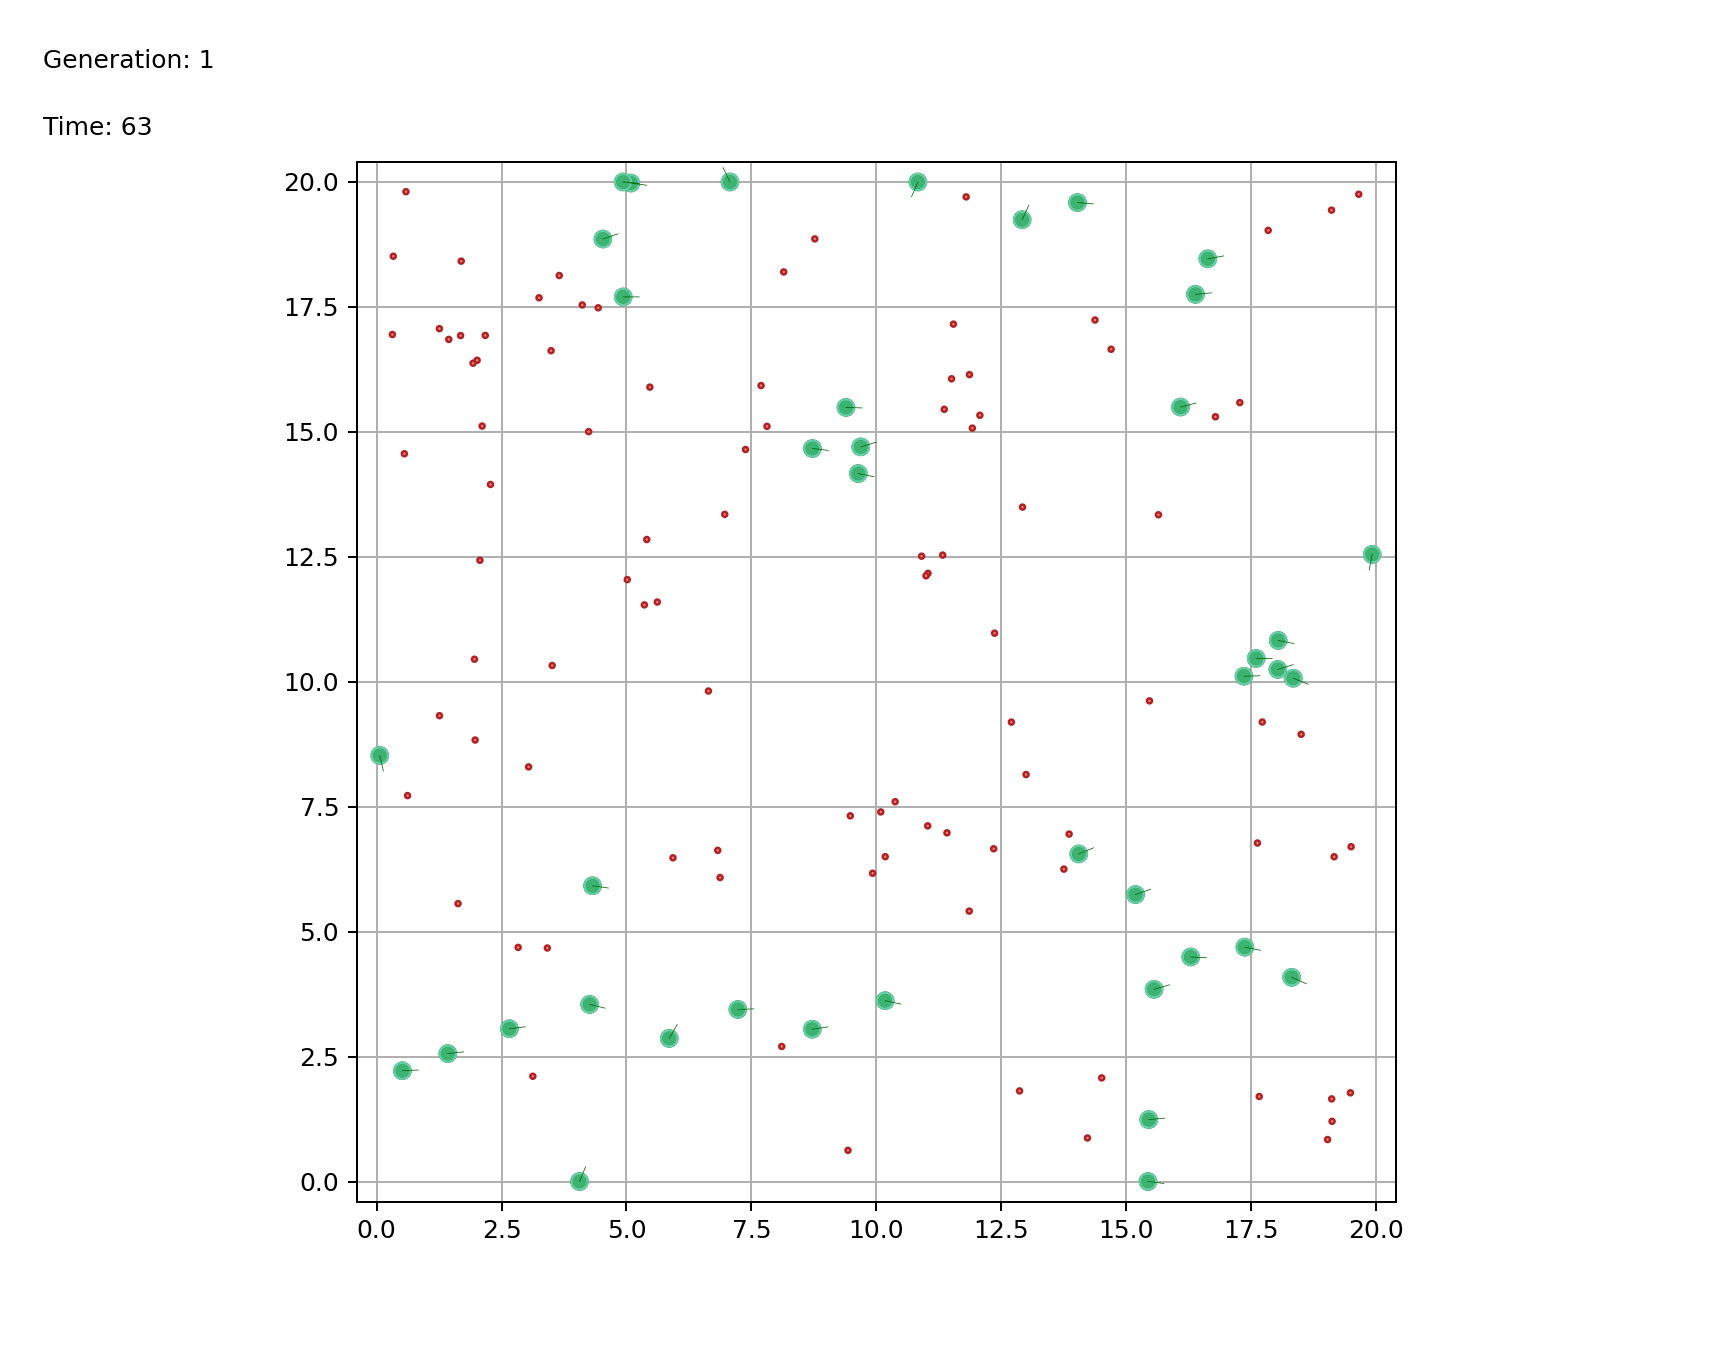
\includegraphics[scale=0.5]{Images/visualizing-the-environment.png}
  \label{fig:візуалізація-середовища}
\end{figure}


Для обробки колізій та ефективного зберігання об’єктів обрано 
просторову структуру даних R-Дерево (R-Tree). 
Ця структура зазвичай використовується для індексації 
багатовимірної інформації, такої як географічні координати, 
прямокутники або багатокутники.
Основною ідеєю цієї структури є ідея групування сусідніх 
об’єктів для представлення їх за допомогою мінімального 
обмежувального прямокутника на наступному вищому рівні дерева. 
Тому і має назву R-Tree, як дерево прямокутників.
Ця структура є корисною для практичних задач із просторовою взаємодією. 
В контексті Python існує бібліотека \verb+rtree+, 
що надає інтерфейс до вже реалізованої бібліотеки на C, 
що встановлюється на систему. 
Таким чином ми забезпечені достатньою швидкістю пошуку, 
зміни та інших маніпуляцій об’єктів у просторі.


Їжа грає ключову роль у процесі виживання та розвитку організмів, 
надаючи потрібний ресурс, що є розподіленим по середовищу. 
Сам об’єкт їжі є точкою з певним числом, 
що задає розмір цієї частинки. 
Кожна ця частинка має певну кількість енергії, 
що задається константно при ініціалізації середовища. 
Сама їжа у середовищі з’являється за ймовірнісним процесом. 
На старті середовища задається параметр для експоненційного розподілу, 
за яким і з’являються частинки у рівномірно вибраній точці середовища.
Також можливо обрати варіант появи їжі лише у певних
областях простору. Це зближує нас із реальною моделлю, оскільки 
природні ресурси, такі як їжа, часто розташовані у скупченнях 
через умови навколишнього середовища. 
Цього можна досягти за допомогою такого методу, як дискова вибірка Пуассона
\cite{bridsonFastPoissonDisk2007}.



%%%%%%%%%%%%%%%%%%%%%%%%%%%%%%%%%%%%%%%%%%%%%%%%%%%%%%%%%%%%%%%%%%%%%%%%%%%%%%%%%%
\section{Організми}

Об’єкт організму репрезентує модель біологічного індивіда, 
що має певний набір характеристик: геном, розмір, швидкість руху, 
прискорення, напрямок, енергетичний рівень, вік.

Геном організму задається парами матриць, 
що слугують вагами та упередженістю нейронної мережі. 
Сам клас самостійно оперує цією структурою. 
Єдина річ, яку потрібно задавати тут це шари нейронної 
мережі та кількість нейронів у них. 
Більша кількість шарів та нейронів призводить до більшого геному.

Кожен організм може думати за допомогою цієї мережі. 
Результат його праці --- це команда на пересування.
Кількість вихідних даних з мережі організму повинна
задаватися типом середовища моделювання.
Для тривимірного простору ми можемо задати шість ступенів свободи.
Все ж для поточної реалізації двовимірного простору
достатньо задати прискорення та зміну кута напряму.

Але кожна команда впирається у фізичні обмеження цього організму. 
Ми обмежуємо його пересування у середовищі задаючи максимальну 
можливу швидкість, прискорення та зміну напряму. 
Це є логічним, оскільки і в реальному житті будь-який 
організм не може змінити свої фізичні характеристики в одну мить. 
А в моделюванні з дискретним часом нам важливо зберегти якусь подібність до реальності.

На швидкості організм не повинен вміти швидко змінювати напрям. 
Саме тому додаємо гальмівний ефект від зміни напряму руху:
\[ v^{(t+1)} = \max(-v_{max}, \min(v_{max}, v^{(t)} + a)) \cdot \frac{1}{1 + d} \]


На обробку інформації про зовнішній світ у організма повинна 
якось змінюватися енергія. 
так ось і буде вона змінюватися за простим законом. 
вводимо коефіцієнт зміни енергії $\mu$ та будемо задавати зміну енергії так:
\[ E^{(t+1)} = E^{(t)} - \mu \cdot \left| \overline{o} \right| \]
Де $\overline{o}$ позначаємо як результат роботи нейронної мережі.

\hide{
Зовнішній світ повинен якось сприйматися організмом.
Наразі нейронні мережі сприймають зображення як матрицю
із закодованими значеннями кольорів.
Зображення по суті є проекцією тривимірних об'єктів.
Наші організми можуть розвиватися як у тривимірному просторі, так
і у двовимірному.
Ідеалістично, фенотип організму не повинен залежати від простору,
у якому він розвивається, але й зір є тісно пов'язаним із середовищем
та ідейно відноситься до об'єкта організму.
Тому кращим рішенням може бути відокремлення механізму зору від організма.
Це надає можливість тестувати довільну кількість таких імплементацій
навіть у одному процесі моделювання.
Такий механізм зору буде диктувати кількість нейронів у вхідному шарі мережі.

Візьмемо підхід, що буде перевикористовувати ідею цифрових зображень.
Зовнішній світ проектується на матрицю фіксованого розміру.
Надалі саме заповнення цієї матриці і залежить від конкретного
способу реалізації зору.
Зменшимо рівень абстракції "зору" до рівня кодування інформації навколо
об'єкта у матрицю фіксованого розміру.
Логічно використовувати набір позицій об'єктів у просторі
та їх фізичні властивості для створення матриці.
Кожен елемент у матриці буде кодувати відстань та напрямок
відносно <<голови>>  організму.
}

Організм повинен якось сприймати навколишнє середовище.
У реалізації Натана Руя \cite{rooyEvolvingSimpleOrganisms}
кожен організм на вхід приймав відстань та напрямок до найближчої
частинки їжу.
Ця модель не зовсім відповідає дійсності, оскільки
прорахунок найближчої цілі, напрям та відстань не отримується просто так.
Як і в житті, ми не бачимо точну відстань до предметів,
а приблизно оцінюємо ці відстань за допомогою орієнтування у просторі,
напруженні м'язів ока або відносній оцінці.
Тому потрібно надати найефективніше найближче сприйняття
до реальності.

Наразі нейронні мережі сприймають зображення як матрицю 
з закодованими значеннями кольорів.
По суті, зображення є проекцією об’єктів у трьох вимірах, тому й
наш механізм зору повинен надавати певну проекцію об'єктів на матрицю.
Ідеалістично, фенотип організму не повинен залежати від середовища, 
у якому він розвивається, але й зір має тісний зв’язок із 
середовищем та ідейно пов’язаний з об’єктом, у якому він знаходиться.
Також наші організми можуть розвиватися як у трьох, так і в двох вимірах.
Тому краще відокремити механізм зору від організму.
Це дозволяє тестувати будь-яку кількість таких імплементацій, 
навіть використовуючи один процес моделювання.
Кількість нейронів у вхідному шарі мережі буде визначена таким механізмом зору.

Виберемо стратегію, яка повторно використовує концепцію цифрових зображень.
Світ навколо організму проектується на матрицю певного розміру.
Заповнення цієї матриці також залежить від конкретного способу реалізації ідеї.
Зменшимо рівень абстракції «зору» до рівня кодування інформації навколо об’єкта в матрицю фіксованого розміру.
Логічно використовувати набір позицій об'єктів у просторі
та їх фізичні властивості для створення матриці.
Кожен елемент матриці закодує напрямок і відстань відносно «голови» організму,
а значення елемента можна подавати як тип об'єкта, де
для їжі ми ставимо одне константне значення, а для інших організмів
на шляху цільового --- інше.

\begin{figure}[ht]
    \centering
    \incfig{наповнення-матриці-для-механізму-зору}
    \caption{Наповнення матриці для механізму зору}
    \label{fig:наповнення-матриці-для-механізму-зору}
\end{figure}


%%%%%%%%%%%%%%%%%%%%%%%%%%%%%%%%%%%%%%%%%%%%%%%%%%%%%%%%%%%%%%%%%%%%%%%%%%%%%%%%
\section{Кодування}

Для генетичних алгоритмів використовують різні методи кодування, 
щоб представити розв'язки задачі в структурі хромосоми або геному. 
Типовими прикладами кодувань є: двійкове кодування, 
цілочисельне кодування, кодування дійсними числами, 
кодування перестановками та кодування значеннями.

Двійкове кодування представляє рішення за допомогою двійкових цифр (0 і 1). 
Якщо простір задачі вимагає дискретних величин, 
краще використовувати цілочисельне кодування, оскільки 
воно використовує цілі числа. Кодування перестановок підходить для 
проблем впорядкування або маршрутизації, 
оскільки воно передбачає розміщення речей або значень у певному порядку. 
У складних проблемних просторах, де певні стани або 
атрибути повинні бути представлені явно, кодування значень, 
також відоме як пряме кодування, передбачає безпосередній запис значень рішення.

У цій реалізації генетичного алгоритму для представлення геному організму 
можна конфігурувати різні можливі кодування. 
Це можливо завдяки правильній структурі коду, 
що дає можливіть швидко змінювати параметри моделі.

Але найкраще використати кодування дійсними числами. 
Перевага кодування в дійсних числах полягає в тому, 
що воно безпосередньо представляє неперервні змінні, що 
робить його особливо придатним для питань, 
пов'язаних з оптимізацією неперервного простору, 
таких як оптимізація ваг нейронних мереж.

Ваги та упередженність нейронної мережі безпосередньо кодуються в 
геномі організму за допомогою цього кодування в дійсних числах. 
Клас \verb+RealValued+ дає можливість кодувати та декодувати 
ваги організму в одновимірний масив геному. 
Для цього ваги та зсуви вирівнюються та об'єднуються. 
Для декодування сплющені масиви повертаються до початкових розмірів.

Завдяки такому кодуванню можна ефективно шукати у неперервному 
просторі оптимальні параметри нейронної мережі організму. 
Через те, що ваги та упередженність за своєю природою 
є дійсними числами, це забезпечує простий та ефективний 
метод оптимізації нейронних мереж. 
Імітуючи еволюцію біологічних організмів і використовуючи 
цей процес для вдосконалення моделей машинного навчання, 
ця методика втілює суть біологічно натхненного навчання.


%%%%%%%%%%%%%%%%%%%%%%%%%%%%%%%%%%%%%%%%%%%%%%%%%%%%%%%%%%%%%%%%%%%%%%%%%%%%%%%%%%
\section{Генетичні оператори}

Генетичні оператори грають величезну роль у зміні 
поведінки організмів та продуктивності генетичного алгоритму. 
Вони дозволяють вивчати можливі рішення проблеми у 
фазовому просторі рішень або ж перевикористати поточні 
варіанти для отримання більш кращого. 
Вибір і конфігурація цих операторів є важливою частиною 
проектування генетичного алгоритму.

Мутація вносить невеликі випадкові зміни в геноми індивідів, 
щоб підтримувати її різноманітність. 
Було запрограмовано різні типи мутації.

\verb+NonUniformMutation+ клас реалізує нерівномірну мутацію, 
яка змінює гени на основі функції, що зменшується з часом, 
сприяючи експлуатації, а не дослідженню в подальшому процесі роботи алгоритму. 
Це дозволяє на кінцевих ітераціях сфокосуватися на отриманні більш 
точних рішень, а ніж дослідженню простору.

\verb+GaussianMutation+ та \verb+UniformMutation+ є Гауссовую мутацією 
та рівномірною мутацією, які вносять зміни з нормального розподілу 
або з рівномірного розподілу відповідно.

Селекція --- це процес вибору особин, або батьків, 
які дадуть потомство у наступному поколінні. 
Клас \verb+TruncationSelection+ реалізує усічений відбір, 
який обирає найкращих $n$ особин на основі їхніх значень пристосованості. 
Цей підхід є простим і ефективним, гарантуючи, 
що для розмноження будуть обрані найбільш пристосовані особини.

Кросинговер --- ще один важливий генетичний оператор. 
Він дозволяє обмінюватися генетичним матеріалом між 
батьківськими особинами, створюючи таким чином потомство.

Клас \verb+SBXCrossover+ реалізує імітований двійковий 
кросинговер (SBX), який імітує поведінку одноточкового кросинговеру 
в генетичних алгоритмах з двійковим кодуванням в контексті кодування 
з дійсними значеннями. 
Він генерує нащадків ближче до батьків 
\cite{debSIMULATEDBINARYCROSSOVER, debSelfadaptiveSimulatedBinary2007}.

Клас \verb+BLXCrossover+ реалізує змішаний кросовер (BLX), 
який створює нащадків у діапазоні, визначеному генами батьків 
і пропорцією, що дозволяє проводити більш значні дослідження \hide{[5, 6].}
\cite{debSIMULATEDBINARYCROSSOVER}.

Клас \verb+ArithmeticCrossover+ генерує нащадків, 
використовуючи лінійну комбінацію генів батьків 
\cite{koraCrossoverOperatorsGenetic2017}.

Клас \verb+UniformCrossover+ реалізує простий рівномірний кросинговер,
де кожен ген нащадка випадковим чином вибирається від одного з батьків
\cite{koraCrossoverOperatorsGenetic2017}.


%%%%%%%%%%%%%%%%%%%%%%%%%%%%%%%%%%%%%%%%%%%%%%%%%%%%%%%%%%%%%%%%%%%%%%%%%%%%%%%%%%
\section{Опис інструментів та збір даних під час моделювання}

Механізм еволюції реалізовано з використанням 
об'єктно-орієнтованого підходу. 
По суті, це конвеєр, який перетворює популяцію організмів 
на наступне покоління. 
Цей процес відбувається в основному за допомогою чотирьох 
ключових кроків: відбору, проходження процесу елітизму, 
кросинговеру та мутації.

Також важливим параметром є ввімкнення процесу помирання 
організмів при досягненні критичної області енергії. 
Таким чином ми можемо отримати стаціонарний генетичний алгоритм, 
який не потребує переходів між популяціями,
змінюючи час на отримання наступної популяції та
кількість осіб у відборі. 
Його основна перевага це постійний процес еволюції, 
помирання індивідів та оптимізації по використанню пам’яті.

Було імплементовано комплексну бібліотеку для зручної роботи 
з дослідженням адаптації організмів до середовища. 
Підхід при її розробці мав на меті легку параметрицію для 
впровадження швидких експериментів по моделюванню життя організмів.

Також варто зазначити, що будь-яка частина програми може 
бути вільно замінена на іншу реалізацію. 
Тобто більш складні середовища можуть бути легко спровадженні у 
цей продукт через його модульність. 
Для дослідження цього проекту було вирішено обмежитися 
одним середовищем та одним типом організмів. 
Це дозволило швидко провести аналіз даних, отриманих за допомогою цієї моделі.

Сам же аналіз повинен здійснюватися по певних даних, які мають бути записані
під час процесу моделювання.
Такий запис повинен бути швидким по часу та займати мало постійної пам'яті,
тому на противагу запису в \verb+CSV+ файли було обрано \verb+Parquet+ тип.
Він має стовпчастий формат файлів для зберігання даних, націлений на обробку
великих масивів. Також забезпечуються ефективні алгоритми стиснення та кодування.

Для аналізу застосовувалися Jupyter Notebooks як середовище виконання коду.
У них відбувалося зчитування даних та візуалізація за допомогою 
бібліотеки для візуалізації даних \verb+plotly+.
Для більш адаптивного аналізу результатів багатьох запусків моделі із
різними параметрами використаний фреймворк \verb+dash+ 
для побудови веб-додатків для візуалізації даних.



%%%%%%%%%%%%%%%%%%%%%%%%%%%%%%%%%%%%%%%%%%%%%%%%%%%%%%%%%%%%%%%%%%%%%%%%%%%%%%
\section{Метрики}

Для аналізу поколінь організмів цілком розумно було б 
використати певний набів метрик, які б показали як 
поводять себе організми у середовищі, якою є їхня 
різноманітність та їх рівень розвитку. 
Використання цих метрик дасть можливість проводити більш 
обґрунтований та деталізований аналіз.

Однією з таких метрик є пристосованість, 
що у даній реалізації є не що інше як рівень енергії у організмі. 
Він надає інформацію про те, наскільки ефективно організм 
використовує доступні йому ресурси та його здатність 
адаптуватися до змін у навколишньому середовищі.

Також ми можемо задати метрику максимального та 
мінімального рівня енергії, що дасть нам більш повну 
інформацію про різноманітність популяції у використанні ресурсів.

Іншою є метрика співвідношення спожитої їжі до кількості 
рухів організму. 
Ця метрика допоможе нам зрозуміти енергоефективність організму, 
показуючи, наскільки ефективно він використовує отримані 
від їжі ресурси для своєї активності. 
Ця метрика обчислюється як відношення 
кількості рухів до кількості спожитих частинок їжі.

\todo[inline]{Metrics formulas}


%%%%%%%%%%%%%%%%%%%%%%%%%%%%%%%%%%%%%%%%%%%%%%%%%%%%%%%%%%%%%%%%%%%%%%%%%%%%%%%%%%
\section{Аналіз впливу параметрів по метрикам}

Дана модель може бути параметризована по:
\begin{enumerate}
  \item Розмірам середовища
  \item Тривалості одного покоління
  \item Типу зору організма
  \item Кількості енергії у частинках їжі та параметрам
    розподілу для генерації цим частинок
  \item Швидкості втрати організмами енергії при русі
  \item Методу відбору, мутації та рекомбінації
  \item Числу осіб, що переходять у наступну популяцію (елітизм)
  \item Розміру генома, що фактично означає кількості прихованих шарів
    та нейронів у них
  \item Кількості їжі, на старті
  \item Чи помиратимуть організми від нестачі енергії
  \item Параметрам нормального розподілу для генерації
    початкових ваг нейронної мережі
\end{enumerate}

%%%%%%%%%%%%%%%%%%%%%%%%%%%%%%%%%%%%%%%
% \todo[inline]{Які параметри розподілу для початкових геномів є кращими?}

Спочатку спробуємо відшукати кращі параметри для розподілу Гауса,
за допомогою якого генеруються початкові ваги нейронних мереж організмів.
Спочатку взято три варіанти для стандартного відхилення: 10, 1 та 0.1.
Математичне сподівання ж залишимо на рівні 0.

\begin{figure}[ht]
  \centering
  \caption{Отримані відношення спожитої їжі до руху при 
  пошуку кращого стандартного відхилення для генерації ваг}
  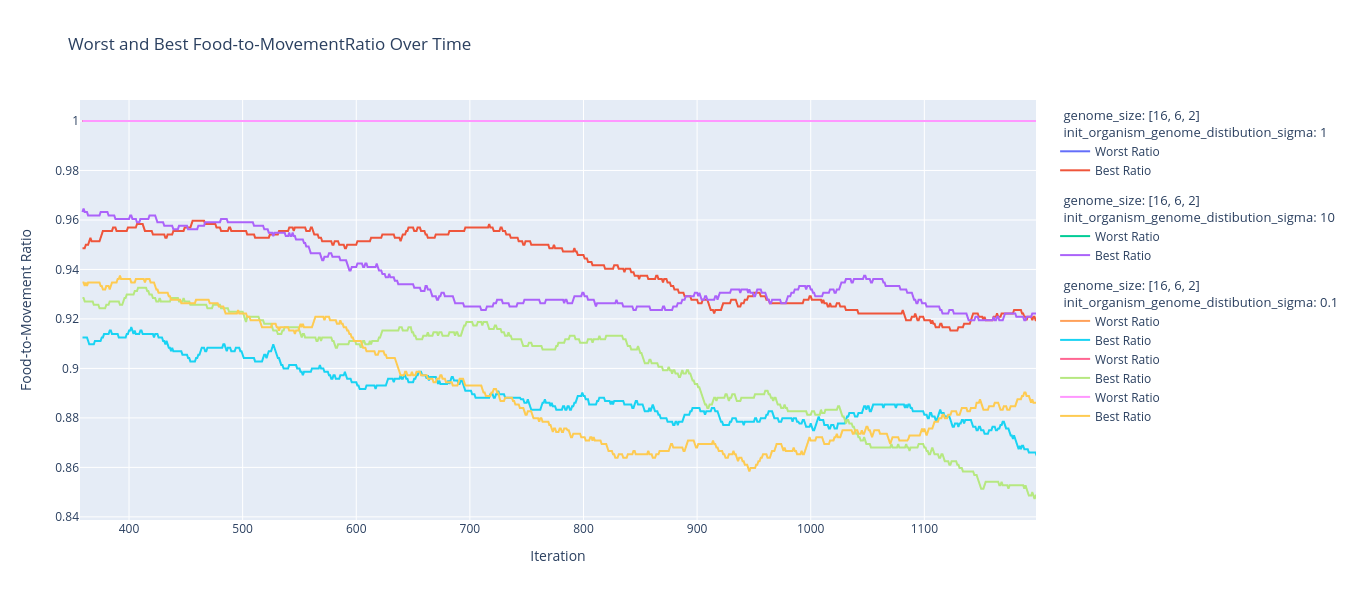
\includegraphics[scale=0.35]{Images/best_sigma_comparing_by_food_to_movement.png}
  \label{fig:отримані-відношення-спожитої-їжі-до-руху-при-пошуку-кращого-стандартного-відхилення-для-генерації-ваг}
\end{figure}

\begin{figure}[ht]
  \centering
  \caption{Рівні енергії при 
  пошуку кращого стандартного відхилення для генерації ваг}
  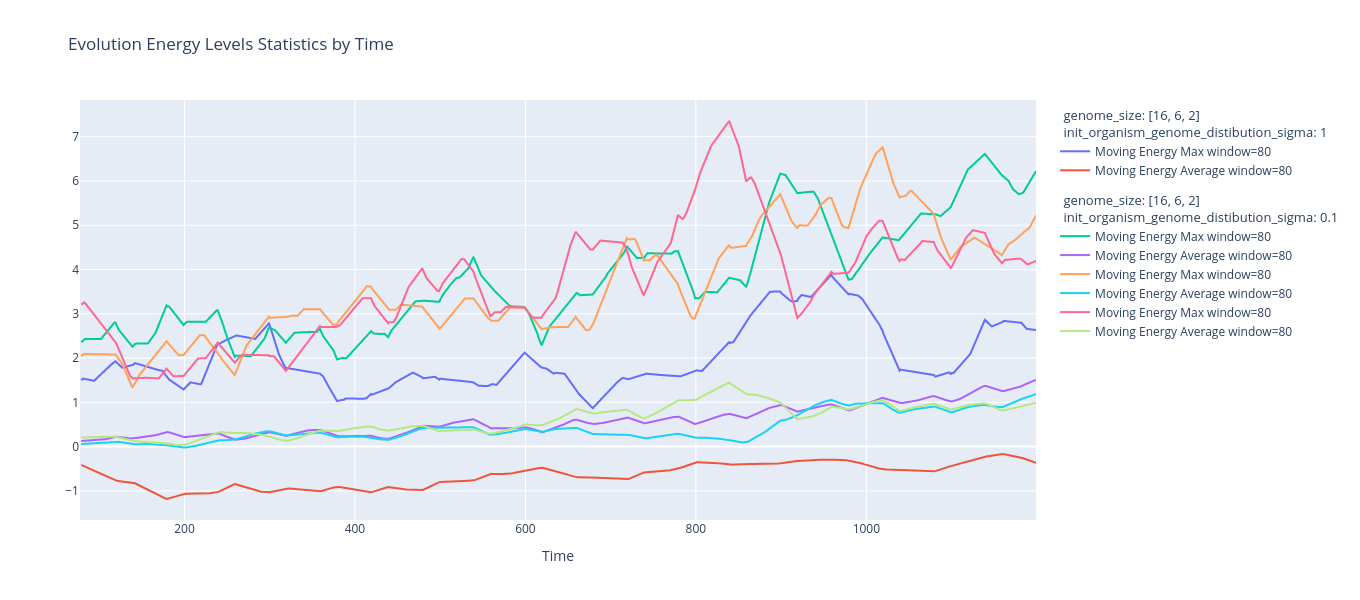
\includegraphics[scale=0.3]{Images/best_sigma_comparing_by_energy_levels.png}
  \label{fig:рівні-енергії-при-пошуку-кращого-стандартного-відхилення-для-генерації-ваг}
\end{figure}

З отриманого графіку \ref{fig:отримані-відношення-спожитої-їжі-до-руху-при-пошуку-кращого-стандартного-відхилення-для-генерації-ваг}
відношення спожитої їжі до руху бачимо помітну різницю
між організмами, що використовували 0.1 як стандартне відхилення, та іншими.
Також середній рівень енергії на графіку 
\ref{fig:рівні-енергії-при-пошуку-кращого-стандартного-відхилення-для-генерації-ваг}
у осіб з 0.1 стандартним відхиленням значно 
відрізняється від осіб з іншим параметром:
середня енергія значно вища, більша за нуль та зростає.
Отже область простору, де ми отримуємо значення геномів
зі стандартним відхиленням у 0.1 надає кращий старт для
життя організмів.



%%%%%%%%%%%%%%%%%%%%%%%%%%%%%%%%
% \todo[inline]{Які методи мутації та кросоверу дають кращий результат?}

Спробуємо підібрати гарну комбінацію методу рекомбінації
та мутації.
Оскільки у генетичних алгоритмах рекомбінація є центральним
елементом еволюції, то почнемо саме з неї.
Візьмемо декілька методів: BLX рекомбінація, Арифметична та
SBX із двома різними параметрами --- 1 та 2.
SBX рекомбінація при параметрі $n = 1$ буде мати
експлуатаційний характер, що дозволить мати пошук у локальній області.
Проаналізуємо графік середнього рівня енергії
по всім організмам впродовж часу.

\begin{figure}[ht]
  \centering
  \caption{Середній рівень енергії при 
  порівнянні методів рекомбінації}
  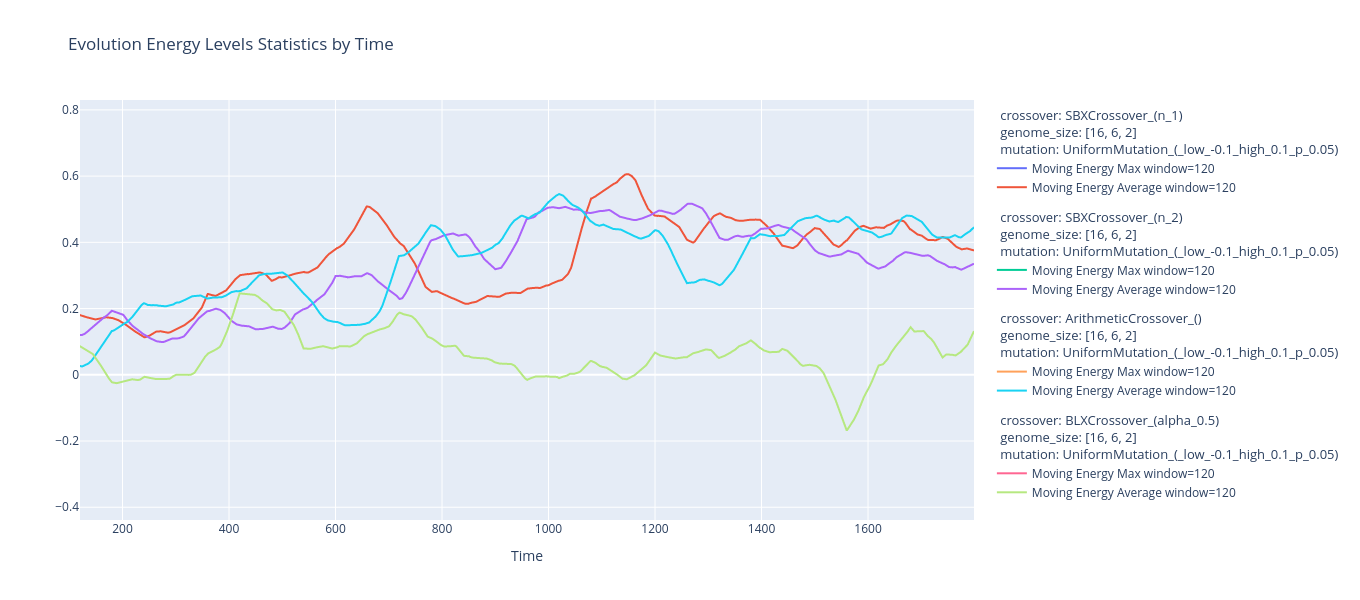
\includegraphics[scale=0.33]{Images/comparing_crossovers_sbx_arithmetic_blx05.png}
  \label{fig:середній-рівень-енергії-при-порівнянні-методів-рекомбінації}
\end{figure}

На графіку \ref{fig:середній-рівень-енергії-при-порівнянні-методів-рекомбінації}
більше всіх виділяється саме BLX рекомбінація із параметром $0.5$.
Він подає гірший результат у порівнянні з двома іншими.
А отже для наших цілей краще надалі використовувати
SBX або ж арифметичну рекомбінацію.

Вплив мутації не є настільки суттєвим та великим.
Під час попереднього моделювання не було помічено
випадку, коли певний метод мутації проявив себе краще, за інші.
Тому було обрано зупинитися на нерівномірній мутації через
її ідею на поліпшенні неявних рішень на завершальних ітераціях
алгоритму.



\todo[inline]{Яка кількість елітів та нащадків дають кращий результат?}



\todo[inline]{чи надає ускладнення форми організму йому переваги у життєдіяльності?}


Візьмемо такий набір кількості прихованих шарів з кількістю нейронів
нейронної мережі:
\begin{itemize}
  \item (6)
  \item (9)
  \item (9, 9)
  \item (18, 9)
\end{itemize}
З використанням 4 секцій дистанції та 4 секцій кута для зору
отримуємо 16 вхідних нейронів у кожній мережі. Також
на вихід маємо видавати два значення. Як результат маємо такий
набір нейронних мереж:
\begin{itemize}
  \item (16, 6, 2)
  \item (16, 9, 2)
  \item (16, 9, 9, 2)
  \item (16, 18, 9, 2)
\end{itemize}

При тестуванні роботи таких мереж отримали наступний графік рівнів енергії
та графік співвідношення спожитої їжі до руху:

\begin{figure}[ht]
  \centering
  \caption{Порівняння різних структур нейронних мереж організмів по максимальній енергії}
  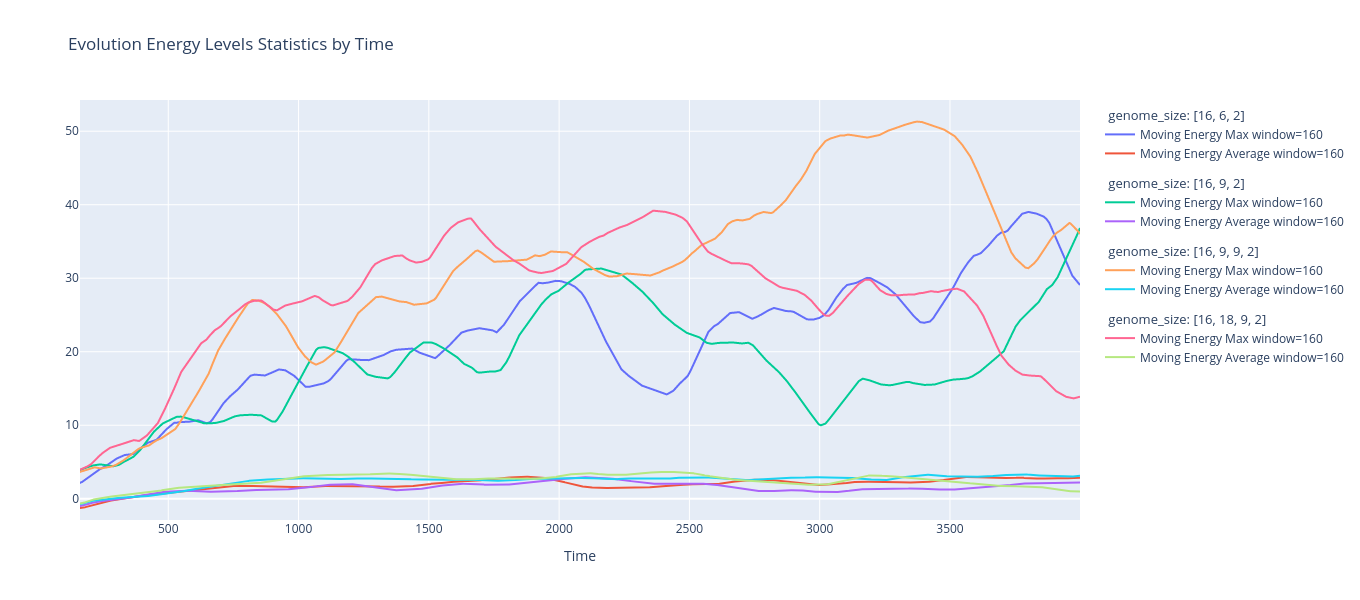
\includegraphics[scale=0.3]{Images/comparing-genomes-at-max-energy.png}
  \label{fig:порівняння-різних-структур-нейронних-мереж-організмів-по-амксимальній-енергії}
% \end{figure}

% \begin{figure}[ht]
  % \centering
  \caption{Порівняння різних структур нейронних мереж організмів по середньому значенню енергії}
  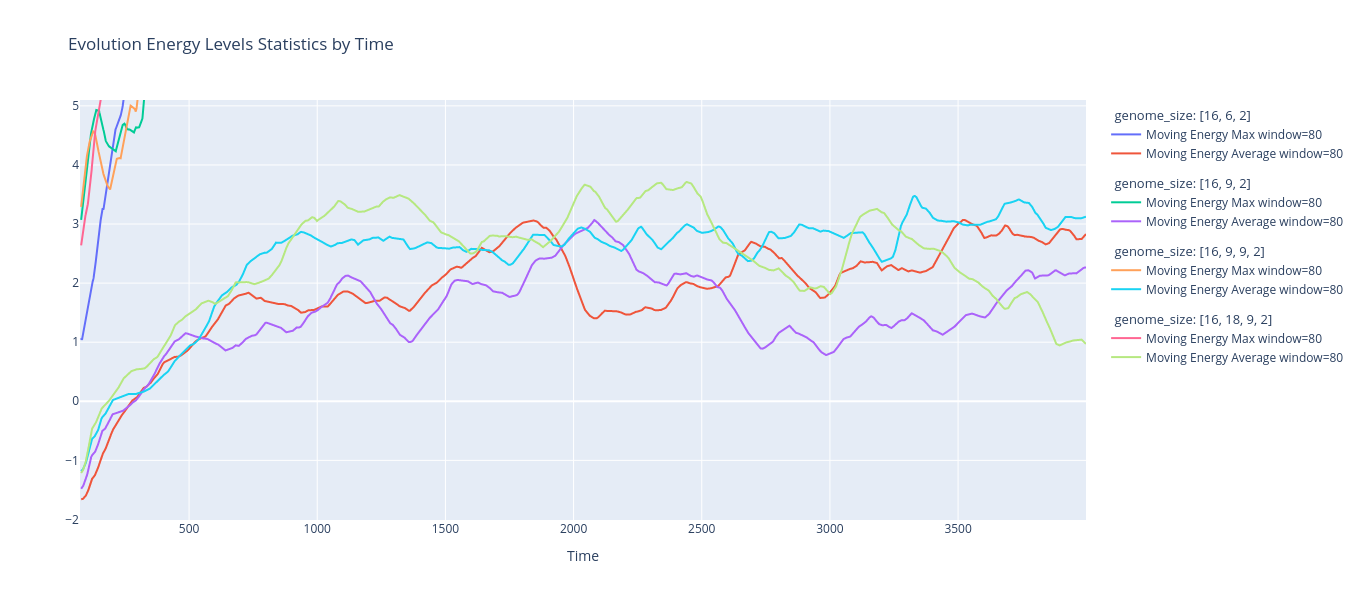
\includegraphics[scale=0.3]{Images/comparing-genomes-at-avg-energy.png}
  \label{fig:порівняння-різних-структур-нейронних-мереж-організмів-по-середньому-значенню-енергії}
\end{figure}

\begin{figure}[ht]
  \centering
  \caption{Порівняння різних структур нейронних мереж організмів по відношенню спожитої їжі до руху}
  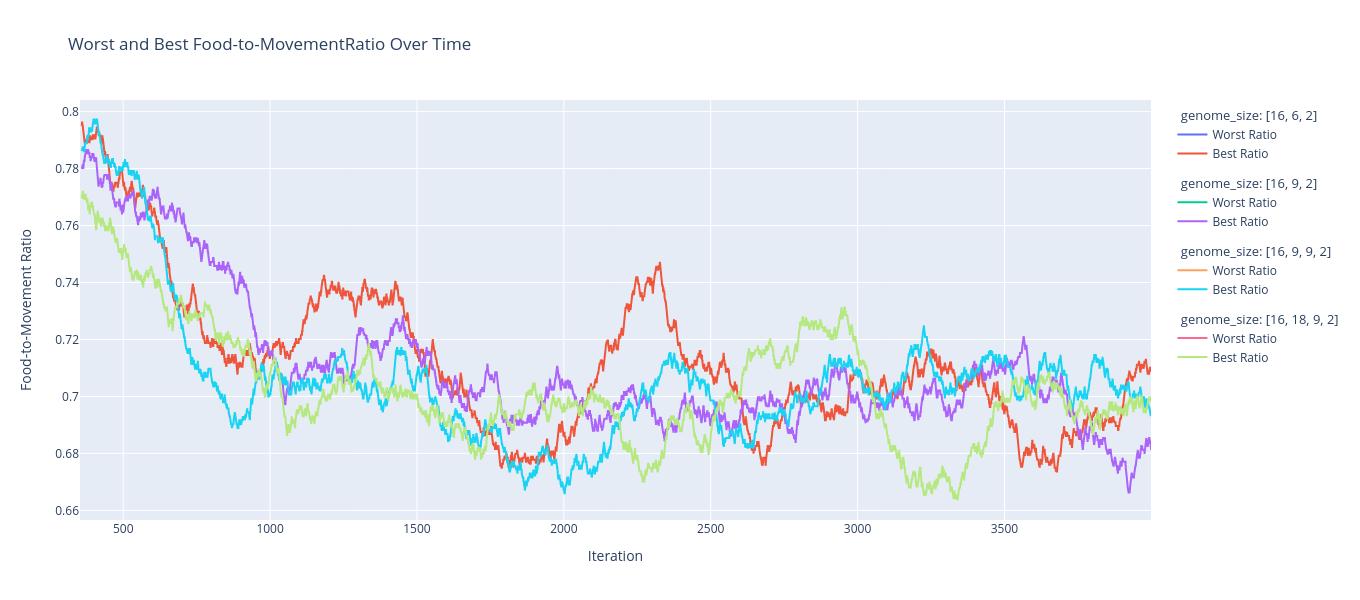
\includegraphics[scale=0.3]{Images/comparing-genomes-at-food-to-movement.png}
  \label{fig:порівняння-різних-структур-нейронних-мереж-організмів-по-відношенню-спожитої-їжі-до-руху}
\end{figure}

З графіку
\ref{fig:порівняння-різних-структур-нейронних-мереж-організмів-по-відношенню-спожитої-їжі-до-руху} 
суттєвої різниці між діями організмів не видно.
А отже навчаються вони досить однаково.

По значенню максимальної кількості енергії
\ref{fig:порівняння-різних-структур-нейронних-мереж-організмів-по-амксимальній-енергії}
схоже, що у індивідів популяції
з більш складнішиою структурою існують індивіди,
що здатні спожити більшу кількість їжі.
Це може означати, що вони розвинули більш досконалі або
ефективні методи використання енергії їжі.
Така поведінка пояснюється збільшенням кількості нейронів,
що могло призвести до покращення здатності вирішувати проблеми
та більш ефективної адаптації до навколишнього середовища.

Однозначно стверджувати, який варіант організмів ми поки не можемо.
Кількість нейронів для простих організмів може бути не на достатньому рівні,
щоб швидко отримати потрібні знання для утилізації частинок їжі.
Спробуємо порівняти із більш складним організмом на рівні
(16, 18, 9, 9, 2) шарів нейронної мережі.


\begin{figure}[ht]
  \centering
  \caption{Порівняння простої та складної структури нейронної мережі організмів по енергії}
  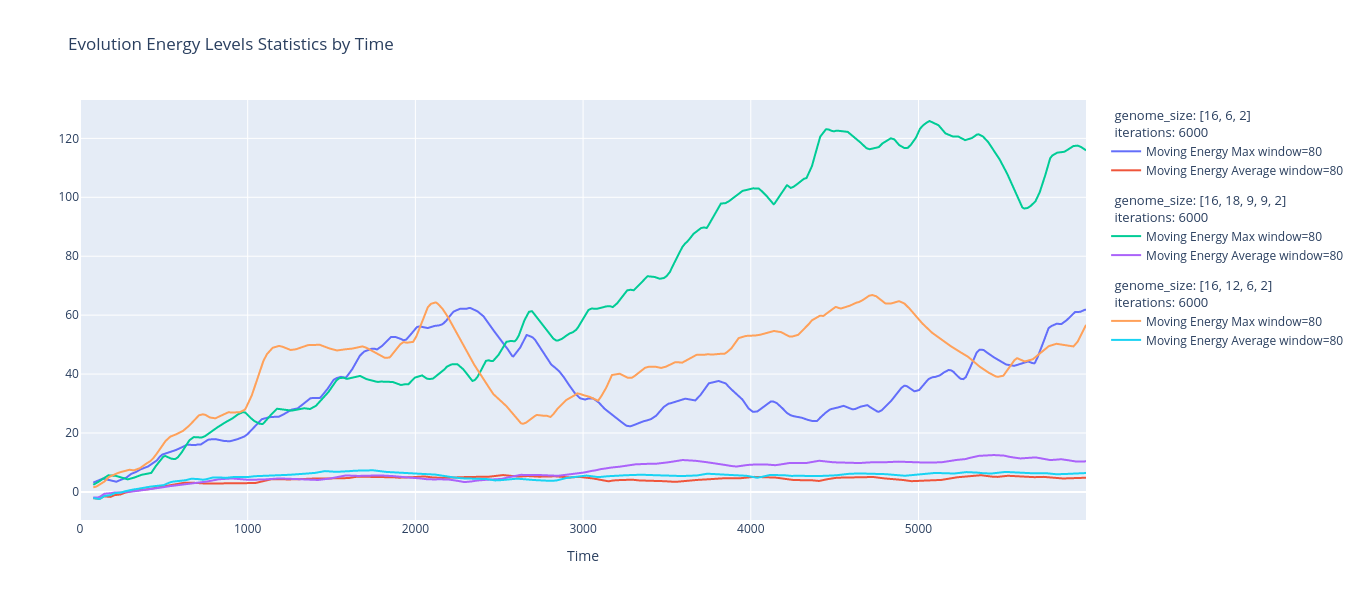
\includegraphics[scale=0.3]{Images/comparing-genomes-energy-levels-complex-is-leader.png}
  \label{fig:порівняння-простої-та-складної-структури-нейронної-мережі-організмів-по-енергії}
\end{figure}

По графіку \ref{fig:порівняння-простої-та-складної-структури-нейронної-мережі-організмів-по-енергії}
можемо проаналізувати, що простіші структури виявилися кращими на початкових
етапах розвитку організмів.
Вони змогли вдосталь пристосуватися для отримання певної кількості енергії
у короткостроковій перспективі.
Але надалі їх розвиток сповільнився.
У той же час складна структура (16, 18, 9, 9, 2) отримувала дані
про навколишній простір та зробила сильний ривок
за рівнем максимальної кількості енергії,
випереджаючи свої простіші аналоги.
По рівню середньої енергії по популяції ця структура має також вищі показники.


На перший погляд, простіші структури отримують більше їжі 
пропорційно до кількості руху та тримають достатній рівень
енергії для виживання на певний період. 
Однак з часом результати роботи як простих, 
так і складних систем змінюються, що 
свідчить про важливість навчання та адаптації в обох типах структур.

\begin{figure}[ht]
  \centering
  \caption{Порівняння простої та складної структури нейронної мережі організмів по відношенню спожитої їжі до руху}
  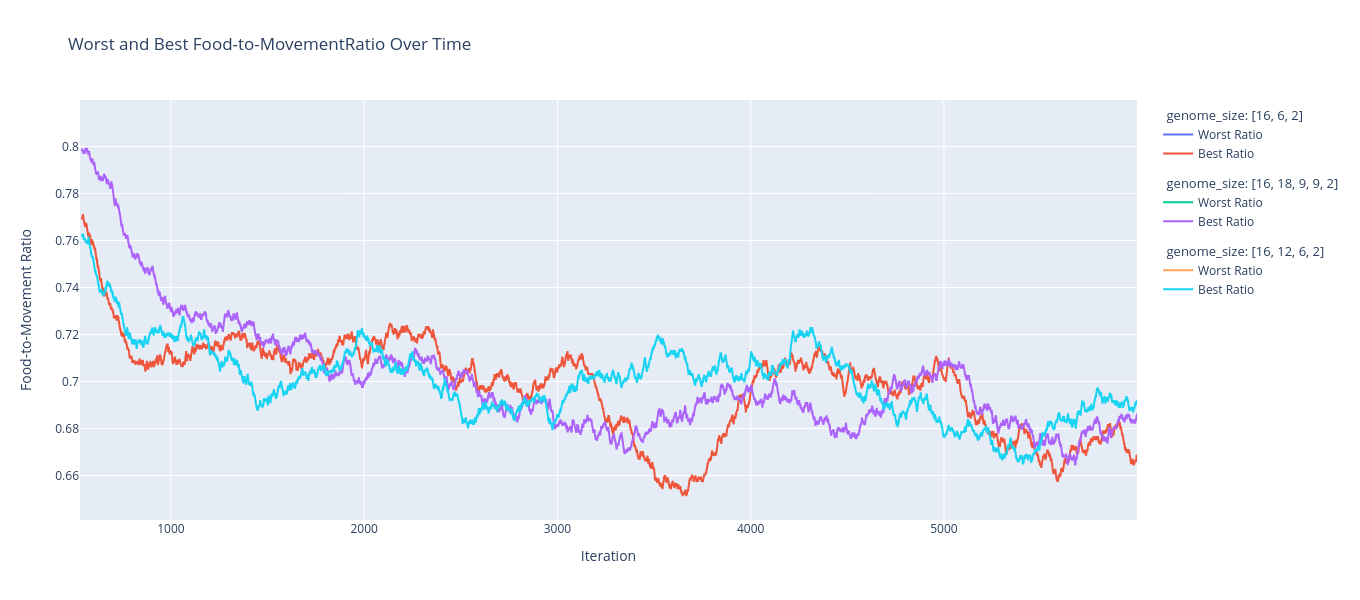
\includegraphics[scale=0.3]{Images/comparing-genomes-food-to-movement-complex-is-leader.png}
  \label{fig:порівняння-простої-та-складної-структури-нейронної-мережі-організмів-по-відношенню-спожитої-їжі-до-руху}
\end{figure}

По графіку відношення спожитої їжі до руху
\ref{fig:порівняння-простої-та-складної-структури-нейронної-мережі-організмів-по-відношенню-спожитої-їжі-до-руху}
чітко видно, як на початкових стадіях розвитку організмів
простіша структура отримує більше їжі, по відношенню до кількості рухів,
але надалі обидва варіанти структур показують перемінний результат.

Такі результати можна пояснити через структурну складність 
конфігурації з більшою кількістю шарів нейронної мережі. 
Через збільшення шарів у мережі організм містить довший геном, 
а отже збіжність популяції з такою структурою може бути повільнішою, 
порівнюючи її з популяцією з меншим геномом.
Оскільки існує менше змінних і менший простір для 
пошуку оптимальних генетичних комбінацій, 
коротші геноми з простішою архітектурою можуть забезпечити 
швидшу адаптацію. 
Як наслідок, менші структури можуть знайти ефективний 
спосіб споживання енергії швидше, ніж їхні складніші аналоги.

Коротший геном дозволив популяції знайти оптимальні рішення 
до отримання все більших запасів енергії за короткий проміжок часу. 
Але популяція з довшим геномом також навчається та 
може вмістити у геном більше інформації для реагування 
на різні події у їхньому житті,
оскільки довший геном забезпечує більшу
різноманітність генетичних комбінацій і, 
як наслідок, більшу можливість для довготривалої адаптації. 
Організмам зі складною структурою може знадобитися більше часу для 
визначення оптимального набору генетичних конфігурацій,
оскільки їх область пошуку є значно більшою. 
Але після цього вони мають потенціал для адаптації до ширшого діапазону 
умов та оптимізації споживання енергії в більшій мірі, ніж простіші структури.
При зміні правил середовища ці знання можуть зіграти свою роль.



%%%%%%%%%%%%%%%%%%%%%%%%%%%%%%%%%%%%%%
% \todo[inline]{ чи спостерігаються паттерни групової свідомості (ройового штучного інтелекту) в поведінці групи?  }


Організми можуть скупчуватися у групи за певних умов.
З мисленого експерменту можна стверджувати, що подібне
скупчення у групи може відбуватися лише при виконанні
як мінімум однієї з двох умов:
\begin{enumerate}
  \item механізм зору в організмів дозволяє їм бачити
    собі подібних;
  \item під час еволюції організми можеть досягти стадії розвитку,
    коли їх поведінка на зовнішні подразники (частинки їжі або інші організми)
    буде мати схожий характер у межах групи.
\end{enumerate}

Хоча й методи розпізнавання та схожа поведінка можуть відігравати важливу роль,
та у формуванні групи можуть діяти й інші процеси.
Наприклад, процес комунікації, спільні способи захисту або добування їжі ---
все може сприяти формуванню групи.
Але такі процеси відносяться до більш складних моделей та реальній моделі
розвитку організмів.

\begin{figure}[ht]
  \centering
  \caption{Утворення групи організмів}
  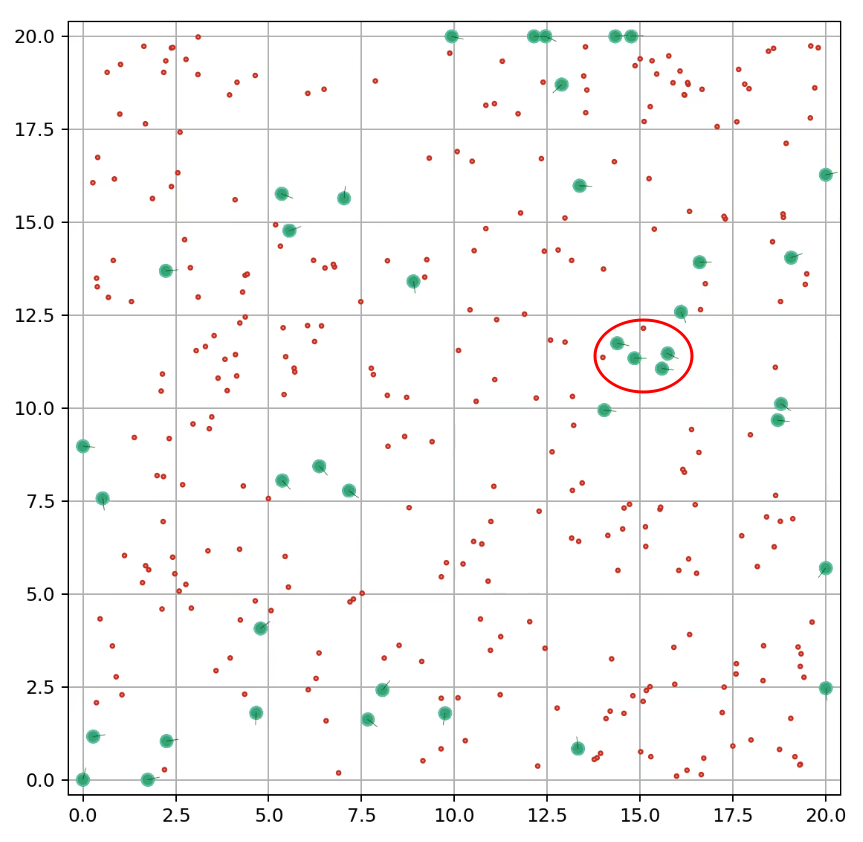
\includegraphics[scale=0.5]{Images/organisms-group-of-4.png}
  \label{fig:утворення-групи-організмів}
\end{figure}

Звичайно, таку складну ідеалізовану модель важко реалізувати,
що беззаперечно дає визнання складності реальних умов.
Та все ж під час спостереження за розвитком організмів під час експерименту
було помічено малі групи індивідів, що рухали за схожим шаблоном.
Часто саме присутність аналогічного організму поряд
давала поштовх змінити курс та слідувати за ним.
Це надає переконливі емпіричні докази групової поведінки,
навіть якщо ці угрупування не дають переваги у такому конкурентному
середовищі.
Часто саме такі групи помирали, оскільки пошук їжі у такому бідному середовищі
вимагає змагання із усіма, навіть із учасниками групи.






%%%%%%%%%%%%%%%%%%%%%%%%%%%%%%%%%%%%%%%%%%%%%%%%%%%%%%%%%%%%%%%%%%%%%%%%%%%%%%%%%%
% \hide{

% Зазвичай третій розділ присвячено опису практичного застосування або 
% експериментальної перевірки аналітичних результатів, одержаних у другому 
% розділі роботи. Втім, це не обов'язкова вимога, і структура основної 
% частини диплому більш суттєво залежить від характеру поставлених завдань. 
% Навіть якщо у вас є певне експериментальне дослідження, але його загальний 
% опис займає дві сторінки, то краще приєднайте його підроздіром у 
% попередній розділ.

% При описі експериментальних досліджень необхідно:

% \begin{itemize}
% \item наводити повний опис експериментів, які проводились, параметрів 
% обчислювальних середовищ, засобів програмування тощо;
% \item наводити повний перелік одержаних результатів у чисельному вигляді для їх можливої 
% перевірки іншими особами;
% \item представляти одержані результати у вигляді таблиць та графіків, 
% зрозумілих людському оку;
% \item інтерпретувати одержані результати з точки зору поставленої задачі 
% та загальної проблематики ваших досліджень.
% \end{itemize}

% У жодному разі не потрібно вставляти у даний розділ тексти 
% інструментальних програм та засобів (окрім того рідкісного випадку, коли 
% саме тексти програм і є результатом проведення експериментів). За 
% необхідності тексти програм наводяться у додатках.

% }
%%%%%%%%%%%%%%%%%%%%%%%%%%%%%%%%%%%%%%%%%%%%%%%%%%%%%%%%%%%%%%%%%%%%%%%%%%%%%%%%%%%

\chapconclude{\ref{chap:practice}}


% Ця робота забезпечила поглиблене вивчення моделі на 
% основі генетичного алгоритму,
% яка імітує еволюцію організмів у віртуальному середовищі. 

Модель репрезентує просту абстракцію реального механізму розвитку організмів,
але не є повним еквівалентом, хоча і поділяє кілька основних концепцій.
Дана модель наслідує механізми виживання та кількості енергії:
реальні біологічні організми споживають певні ресурси, що надають їм можливість
виживати. Цей принцип є фундаментальним у такій моделі.
Подібно до справжньої біологічної еволюції, 
модель використовує генетичні алгоритми для імітації концепцій 
природного відбору, мутацій та успадкування. 
Нейронна мережа є абстрактною картиною того,
як реальні істоти використовують свій генетичний код
для створення складних дій та функцій.
Те, як нейронна мережа використовується
для відтворення процесу <<мислення>> організму,
схоже на те, як реальні тварини використовують
свій мозок для взаємодії з навколишнім середовищем.
Однак важливо зазначити, що спрощення та абстракції, 
необхідні для комп'ютерного моделювання означають, 
що дана модель не є ідеальним відображенням реального світу
через обмеження у: сенсорах, спрощеному середовищі,
відсутності росту, складності геному.


Дослідження виявило динамічний зв'язок між складністю геному, 
швидкістю еволюції та довгостроковою адаптацією. 
Підібрані гарні параметри для старту моделювання та механізми
еволюції.
Було показано, що організми з простішою генетичною архітектурою адаптуються 
швидше через менший простір рішень. 
Однак, незважаючи на більш повільну початкову еволюцію, 
індивіди зі складнішою архітектурою геному демонстрували кращий потенціал 
для довгострокової адаптації.
Цікаво, що, незважаючи на простоту моделі, було виявлено
зачатки розвитку груп у популяції. 

% Дослідження також висвітлило труднощі, пов'язані з дефіцитом 
% ресурсів, оскільки групи часто гинули через труднощі в отриманні їжі, 
% що підкреслює компроміс між соціальною поведінкою 
% та конкурентною боротьбою за ресурси. 
% Це узгоджується з тенденціями, що спостерігаються в біологічних системах, 
% і підкреслює необхідність додаткових досліджень еволюції кооперативних 
% або взаємовигідних дій у відповідь на екологічні обмеження.

% Результати дослідження демонструють потужність генетичних алгоритмів 
% у відтворенні складних біологічних процесів, 
% які є результатом простих еволюційних механізмів. 
% Проект підкреслює корисність еволюційних обчислень як інструменту 
% для розуміння біологічної еволюції та 
% вдосконалення складних систем штучного інтелекту.

% Загалом, це дослідження закладає основу для майбутніх 
% досліджень еволюційної динаміки, зокрема, 
% впливу змін умов навколишнього середовища та генетичної складності 
% на адаптацію та стратегії виживання організмів.


% \todo[inline]{
% - чи відображає модель з достатньою точністю поведінку реальних систем? (так, навести приклади, якщо зможете)

% - чи надає ускладнення форми організму йому переваги у життєдіяльності? (парадоксально, але не завжди - прості, але швидкі і прожерливі організми швидше накопичують вагу)

% - чи спостерігаються паттерни групової свідомості (ройового штучного інтелекту) в поведінці групи? (про певні залежності можна говорити, але потрібні додаткові обчислювальні експерименти. якщо щось спостерігалося - можна вказати)
% }



% Створюємо висновки \conclusions
%!TEX root = ../thesis.tex
% створюємо Висновки до всієї роботи

\conclusions

% Ця робота забезпечила поглиблене вивчення моделі на 
% основі генетичного алгоритму,
% яка імітує еволюцію організмів у віртуальному середовищі. 

% Загальні висновки до роботи повинні підсумовувати усі ваші досягнення у 
% даному напрямку досліджень.

% За кожним пунктом завдань, поставлених у вступі, у висновках повинен 
% міститись звіт про виконання: виконано, не виконано, виконано частково (І 
% чому саме так). Наприклад, якщо першим поставленим завданням у вас іде 
% <<огляд літератури за тематикою досліджень>>, то на початку висновків ви 
% повинні зазначити, що <<у ході даної роботи був проведений аналіз 
% опублікованих джерел за тематикою (...), який показав, що (...)>>. Окрім 
% простої констатації про виконання ви повинні навести, які саме результати 
% ви одержали та проінтерпретувати їх з точки зору поставленої задачі, мети 
% та загальної проблематики.

% \todo[inline]{висновки про поставленні завдання}

Було проведено огляд по доступним джерелам по темі моделей розвитку
організмів, з яких було виведено вимоги до даної моделі.
Також огляд по джерелам еволюційних алгоритмів підштовхнув до розширення
загальності генетичного алгоритму, використаного у даній роботі.

У другому розділі було сформовано принцип роботи із нейронними мережами
у моделі та вимоги до побудови цієї моделі даної роботи.

У третьому розділі описано реалізацію моделі, а також оглянуто результати
її роботи. 

% В ідеалі загальні висновки повинні збиратись з висновків до кожного 
% розділу, але ідеал недосяжний. :) Однак висновки не повинні містити 
% формул, таблиць та рисунків. Дозволяється (та навіть вітається) 
% використовувати числа (на кшталт <<розроблена методика дозволяє підвищити 
% ефективність пустопорожньої балаканини на $2.71\%$>>).

% Наприкінці висновків необхідно зазначити напрямки подальших досліджень: 
% куди саме, як вам вважається, необхідно прямувати наступним дослідникам у 
% даній тематиці.





% \todo[inline]{
% - чи відображає модель з достатньою точністю поведінку реальних систем? (так, навести приклади, якщо зможете)
% }

Ця робота забезпечила поглиблене вивчення моделі на 
основі генетичного алгоритму,
яка імітує еволюцію організмів у віртуальному середовищі. 
Модель репрезентує просту абстракцію реального механізму розвитку організмів,
але не є повним еквівалентом, хоча і поділяє кілька основних концепцій.
Дана модель наслідує механізми виживання та кількості енергії:
реальні біологічні організми споживають певні ресурси, що надають їм можливість
виживати. Цей принцип є фундаментальним у такій моделі.
Подібно до справжньої біологічної еволюції, 
модель використовує генетичні алгоритми для імітації концепцій 
природного відбору, мутацій та успадкування. 
Нейронна мережа є абстрактною картиною того,
як реальні істоти використовують свій генетичний код
для створення складних дій та функцій.
Те, як нейронна мережа використовується
для відтворення процесу <<мислення>> організму,
схоже на те, як реальні тварини використовують
свій мозок для взаємодії з навколишнім середовищем.
Однак важливо зазначити, що спрощення та абстракції, 
необхідні для комп'ютерного моделювання означають, 
що дана модель не є ідеальним відображенням реального світу
через обмеження у: сенсорах, спрощеному середовищі,
відсутності росту, складності геному.



% Згідно з дослідженням, існує постійний зв’язок між складністю геному, швидкістю еволюції та довгостроковою адаптацією. 
% % Хороші параметри для початку моделювання та еволюції
% Організми з простішою генетичною архітектурою були показані здатними адаптуватися швидше через менший простір рішень. 
% Незважаючи на більш повільну початкову еволюцію, люди зі складнішою структурою геному були більш адаптованими в довгостроковій перспективі.
% Цікаво, що незважаючи на простоту моделі, було виявлено початки розвитку груп у популяції. 

% Дослідження виявило динамічний зв'язок між складністю геному, 
% швидкістю еволюції та довгостроковою адаптацією. 
% Підібрані гарні параметри для старту моделювання та механізми
% еволюції.
% Було показано, що організми з простішою генетичною архітектурою адаптуються 
% швидше через менший простір рішень. 
% Однак, незважаючи на більш повільну початкову еволюцію, 
% індивіди зі складнішою архітектурою геному демонстрували кращий потенціал 
% для довгострокової адаптації.
% Цікаво, що, незважаючи на простоту моделі, було виявлено
% зачатки розвитку груп у популяції. 

% Дослідження також висвітлило труднощі, пов'язані з дефіцитом 
% ресурсів, оскільки групи часто гинули через труднощі в отриманні їжі, 
% що підкреслює компроміс між соціальною поведінкою 
% та конкурентною боротьбою за ресурси. 
% Це узгоджується з тенденціями, що спостерігаються в біологічних системах, 
% і підкреслює необхідність додаткових досліджень еволюції кооперативних 
% або взаємовигідних дій у відповідь на екологічні обмеження.

Результати дослідження демонструють потужність генетичних алгоритмів 
у відтворенні складних біологічних процесів, 
які є результатом простих еволюційних механізмів. 
Проект підкреслює корисність еволюційних обчислень як інструменту 
для розуміння біологічної еволюції та 
вдосконалення складних систем штучного інтелекту.



% \todo[inline]{
% - чи надає ускладнення форми організму йому переваги у життєдіяльності? (парадоксально, але не завжди - прості, але швидкі і прожерливі організми швидше накопичують вагу)
% }

% Згідно з дослідженням, існує динамічний зв'язок між складністю геному, 
% швидкістю еволюції та довготривалою адаптацією. 
% Було продемонстровано, що організми з простішою генетичною 
% архітектурою адаптуються швидше, оскільки простір рішень є меншим. 
% Однак особини зі складнішою архітектурою геному мають 
% вищий потенціал для довготривалої адаптації, 
% незважаючи на повільнішу еволюцію на початковому етапі.

Дослідження розкриває складні взаємозв'язки між складністю геному 
організму, швидкістю еволюції та здатністю до довготривалої адаптації 
до навколишнього середовища. 
Отримані дані свідчать про те, 
що організми з більш простою генетичною структурою здатні 
швидше адаптуватися. 
Менший простір рішень уможливлює швидший відбір і 
застосування вигідних генетичних особливостей, 
що може бути причиною такої швидкості. 
Нижчий рівень складності таких геномів полегшує організмам 
швидке розпізнавання та набуття ознак, 
які допоможуть їм вижити в поточному середовищі, 
що сприяє швидшій еволюції.

Це дослідження також показує, 
що складніша геномна архітектура дає значну перевагу з 
точки зору потенціалу довгострокової адаптивності, 
навіть якщо спочатку вона розвивається повільніше. 
Складний геном має більше змінних, 
що розширює простір пошуку генетичного алгоритму 
і збільшує ймовірність виявлення різних якостей, 
які можуть бути корисними. 
Ці складнощі дають більший простір для адаптації, 
збільшуючи можливості цих видів реагувати на навколишнє середовище 
і пристосовуватися до нього, 
навіть якщо вони спочатку сповільнюють темп еволюції.

% Результати дослідження привертають увагу до потенційного конфлікту 
% між здатністю до довгострокової еволюції та 
% короткостроковою адаптивністю. 
% Істоти зі складнішими генетичними системами мають більшу 
% здатність до довгострокової адаптації, 
% навіть якщо простіші істоти можуть процвітати на ранніх стадіях 
% завдяки своїй здатності швидко реагувати на нагальні екологічні обмеження.
% Незважаючи на повільніший темп початкової еволюції, 
% ці складні істоти можуть перевершити своїх простіших побратимів у 
% довгостроковій перспективі завдяки постійному використанню широкої 
% зони генетичного пошуку та здатності пристосовуватися до 
% різноманітних мінливих умов навколишнього середовища.

Ці відкриття суттєво вплинуть на наші знання про еволюцію, 
адаптацію та роль складності геному в цих процесах. 
Це спонукає нас переосмислити еволюцію як процес, 
що врівноважує короткострокові вигоди швидкої адаптації 
з довгостроковими перевагами генетичного різноманіття 
і складності, а не як просту боротьбу за виживання.

% Згідно з дослідженням, існує постійний зв’язок між складністю геному, 
% швидкістю еволюції та довгостроковою адаптацією. 
% Хороші параметри для початку моделювання та еволюції
% організми з простішою генетичною архітектурою були 
% показані здатними адаптуватися швидше через менший простір рішень. 
% Незважаючи на більш повільну початкову еволюцію, 
% особи зі складнішою структурою геному були більш адаптованими 
% в довгостроковій перспективі.

% \todo[inline]{
% - чи спостерігаються паттерни групової свідомості (ройового штучного інтелекту) в поведінці групи? (про певні залежності можна говорити, але потрібні додаткові обчислювальні експерименти. якщо щось спостерігалося - можна вказати)
% % }

Цікаво, що незважаючи на простоту моделі, 
було виявлено початки розвитку груп у популяції. 
Під час експерименту було спостережено за 
розвитком організмів у малих групах людей, 
які рухалися за схожим шаблоном.
Часто саме наявність подібного організму поруч 
мотивувала змінити курс і слідувати за ним.
Це дає переконливі емпіричні докази групової поведінки, 
навіть якщо ці угрупування не надають переваг у 
такому конкурентному середовищі.
Такі групи часто гинули, оскільки пошук їжі в 
такому бідному середовищі вимагає змагання з усіма, 
навіть із членами групи.

% \todo[inline]{напрямки подальших досліджень}

Розроблена тут модель є відносно простою з точки зору 
складності організмів і навколишнього середовища. 
Майбутні дослідження можуть включати розробку більш складних 
організмів з розширеними можливостями або включення 
додаткових факторів навколишнього середовища. 
Це дозволило б вивчати більш складні взаємодії та поведінку.

Виникнення групової поведінки в певних ситуаціях 
у даній моделі є цікавим напрямком для майбутніх досліджень. 
Можна дослідити умови, за яких виникає групова поведінка, 
і її вплив на виживання та пристосованість організмів.

Хоча вивчено деякі ефекти зміни складності нейронної мережі, 
що використовується організмами, існує потенціал для дослідження 
більш досконалих архітектур нейронних мереж. 
Це включає використання згорткових або рекурентних нейронних мереж, 
які можуть запропонувати організмам різні можливості.

У поточній моделі середовище є статичним. 
Майбутні дослідження можуть дозволити середовищу 
еволюціонувати разом з організмами, 
що призведе до гонки між адаптацією та мінливими умовами.

Загалом, це дослідження закладає основу для майбутніх 
досліджень еволюційної динаміки, зокрема, 
впливу змін умов навколишнього середовища та генетичної складності 
на адаптацію та стратегії виживання організмів.


% Додаємо бібліографію
% Якщо ви володієте магією bibtex-у, використовуйте її та модифікуйте файл 
% з бібліографією відповідним чином
%!TEX root = ../thesis.tex
% створюємо список використаної літератури
\begin{thebibliography}    
    \bibitem{sad} 
    asda

    \bibitem{dca}
    asd [Електронний ресурс]. --- Режим доступу: \url{dsf}.

@Book{ Luke2013Metaheuristics, 
       author =    { Sean Luke }, 
       title =     { Essentials of Metaheuristics },
       edition =   { second },
       year =      { 2013 }, 
       publisher = { Lulu },
       note =      { Available for free at http://cs.gmu.edu/$\sim$sean/book/metaheuristics/ } 
     }
 
\end{thebibliography}


%\bibliographystyle{ugost2008}
%\bibliography{thesis}

% Створюємо додатки (дивись у файли додатків для необхідних пояснень)
% Якщо ви маєте меншу або більшу кількість додатків, модифікуйте наступні 
% рядки відповідним чином
% Якщо ви не маєте додатків, просто закоментуйте наступні рядки
%!TEX root = ../thesis.tex
\append{Тексти програм}
\label{appendix:A}

Тексти інструментальних програм для проведення експериментальних досліджень необхідно 
виносити у додатки.

\section{Програма 1}

Зауважте, як змінилась нумерація.
%!TEX root = ../thesis.tex
\append{Великі рисунки та таблиці}
\label{appendix:B}

Якщо результати вашої роботи описуються величезними рисунками і таблицями 
(один аркуш та більше) у незліченній кількості, іх також необхідно 
виносити у додатки.

% (Зробити ще два додатки -- приклади відгуку та рецензії)


% Нарешті
\end{document}
